\chapter{Correctness in Transformation Networks
    \pgsize{20 p.}
}
%% PLANNED STRUCTURE:
% Introduce consistency, preservation, app function Informally
% Discuss notions of correctness and identify what we are interested in
% Provide an appropriate formalism to describe that
% Derive research questions from the formalization (compatibility, synchronization, orchestration, probability of errors)

\todo{Add somewhere (best at definition of binary): We consider binary transformation, but, finally, even with multiary transformation, we want to be able to combine them to networks}

In this chapter, we will first discuss a rather informal notion of consistency and its preservation. It is supposed to discuss the different dimensions in which consistency and its preservation can be considered to then discuss how \emph{correctness} can be reasonably defined.
After identifying the correctness notion that is relevant in the context of our assumption, we define a suitable formal notion of consistency.
We then formally define correctness for that notion of consistency.
This chapter thus answers the following research question:
\researchquestionrepeat{rq:correctness:notions}

%%
%% CONSISTENCY NOTIONS
%%
\section{Notions of Consistency and its Preservation}

We begin with a informal discussion of different ways to consider consistency. This especially involves \emph{intensional} and \emph{extensional} notions of consistency as well a \emph{monolithic} and \emph{modular} notions.


\subsection{Intensional and Extensional Consistency Notions}

\mnote{Intensional / extensional consistency}
When we consider a set of models, we would intuitively say that it is consistent if it fulfills some kind of constraints.
Defining these constraints to derive or check whether a given set of models is consistent constitutes an \emph{intensional specification} of consistency, because the set that contains all consistent models is intensionally represented by these constraints and can be derived from it.
We can consider a set of constraints as a predicate, i.e. a Boolean-valued function $I$, which indicates whether a model set $\modelset{m}$ fulfills the constraints $I: \metamodelsetinstanceset{M} \mapsto \setted{true, false}$. Then we can say that:
\begin{align*}
    \modelset{m} \consistenttomath I \equivalentperdefinition I(\modelset{m}) = true
\end{align*}
On the contrary, one can also enumerate the consistent sets of models, thus a set of models is considered consistent if it is contained in that enumeration.
This constitutes an \emph{extensional specification} of consistency.
Given such an enumeration $E = \setted{\modelset{m} \mid \modelset{m} \mathtext{is consistent}}$, we can say that:
\begin{align*}
    \modelset{m} \consistenttomath E \equivalentperdefinition \modelset{m} \in E
\end{align*}

\mnote{Equivalence intensional / extensional specifications}
It is easy to see that both kinds of specifications are equivalent. For each intensional specification the extensional one can be derived by enumerating all models that fulfill the constraints:
\begin{align*}
    E = \setted{\modelset{m} \mid I(\modelset{m}) = true}
\end{align*}
An extensional specification could also be transferred to an intensional one by defining constraints that are fulfilled by exactly the enumerated instances:
\begin{align*}
    I(\modelset{m}) \mapsto 
    \begin{cases} 
        true, & \modelset{m} \in E\\
        false, & \modelset{m} \not\in E\\
    \end{cases}
\end{align*}
For us, however, it will only be relevant that an intensional specification can be transformed into an extensional one.

\mnote{Extensional specifications for theoretical considerations}
A developer who defines consistency, usually wants to use an intensional specification, as tools like transformation languages usually allow the specification of constraints rather than enumerating consistent instances. This is due to the fact that he or she cannot explicitly enumerate all consistent models but only define constraints that allow to derive them.
However, from a theoretical perspective we prefer to consider extensional specifications, because they allow to apply set theory.
Due to the fact that each intensional specification can be transformed into an extensional one, we can make theoretical statements about extensional specifications that also hold for intensional ones.
In the following, we always consider extensional specifications, unless otherwise stated.
So we define the models that are considered consistent in terms of relations, which we also call \emph{\glspl{consistency relation}}.


\subsection{Monolithic and Modular Consistency Notions}

\mnote{Intuitive notion of monolithic and modular}
Consistency, be it specified intensionally or extensionally, can be considered in an either monolithic or modular way.
Having a single specification of consistency for an arbitrary number of models constitutes a \emph{monolithic} notion of consistency.
Like discussed for intensional and extensional consistency specification, this can be expressed by a set of models fulfilling constraints or being contained in a relation.
On the other hand, a \emph{modular} notion of consistency considers several relations between subsets of the relevant models and all together define when models are to be considered consistent.

\mnote{Example for modular specification}
For an extensional notion of consistency between three models $\model{m}{1}, \model{m}{2}, \model{m}{3}$, a modular specification could manifest in three relations $\consistencyrelation{R}{1,2}, \consistencyrelation{R}{1,3}, \consistencyrelation{R}{2,3}$ defining the model pairs that are considered consistent.
If two models are consistent to one of the relations, we can say that they are \emph{locally} consistent to that relation.
However, we are interested in whether models are \emph{globally} consistent to all these relations, so we can say that:
\begin{align*}
    & \model{m}{1}, \model{m}{2}, \model{m}{3} \mathtext{are consistent} \equivalentperdefinition \\
    & \formulaskip 
    \tupled{\model{m}{1},\model{m}{2}} \in \consistencyrelation{R}{1,2} \land \tupled{\model{m}{1},\model{m}{3}} \in \consistencyrelation{R}{1,3} \land \tupled{\model{m}{2},\model{m}{3}} \in \consistencyrelation{R}{2,3}
\end{align*}
%
\mnote{Modular specification also for non-binary relations}
In the example, we considered a modular notion based on binary relation. Such a modular notion, however, can also be based on multiple n-ary relations. For reasons of simplicity, we stick to modular notions of binary relations, although the considerations can be easily transferred to n-ary ones.


\subsection{Consistency Preservation}

\mnote{Consistency preservation keeps models in a relation}
Consistency preservation is the process of ensuring that models stay consistent.
Based on a notion of \glspl{consistency relation} that describe when models are to be considered consistent, this process ensures that models stay in that relation. 
If models get changed such they that are not in the relation anymore, consistency preservation updates the models such that they, again, are in that relation.
In consequence, consistency preservation is always relative to relations defining a consistency.

\mnote{Consistency preservation can be considered a function}
Consistency preservation can be considered a function $\function{Cp}$ that takes (potentially inconsistent) models and returns a consistent set of models:
\begin{align*}
    \function{Cp}(\modelset{m}) \mapsto \modelset{m'}
\end{align*}
We would require from that function that: $\forall \modelset{m} : \function{Cp}(\modelset{m}) \mathtext{is consistent}$.
The definition of \emph{is consistent} depends on whether we rely on a monolithic or modular notion of consistency.
Thus it may require the models to be in one or multiple relations.
For example, given a monolithic relation $\consistencyrelation{R}{}$, $\function{Cp}$ is supposed to fulfill that: $\forall \modelset{m} : \function{Cp}(\modelset{m}) \in \consistencyrelation{R}{}$.
Since these functions define how consistency is preserved, we also call them \emph{\glspl{consistency preservation rule}}

\mnote{Modular consistency preservation is not independent}
Like for the proposed notion of consistency, we can also consider consistency preservation in an either monolithic or modular way.
With a modular notion of consistency preservation, we may have multiple \glspl{consistency preservation rule} that preserve consistency, each of them for a \gls{consistency relation} that defines consistency for a subset of the involved models.
Unlike for the relations defining consistency, which can be evaluated independently to identify whether models are consistently, the functions, i.e. \glspl{consistency preservation rule}, cannot be evaluated independently.
If each function is executed independently, they return new models that may need to be merged. 
Imagine two functions $\function{Cp}_{1,2}$ and $\function{Cp}_{2,3}$ that preserve consistency for relations $\consistencyrelation{R}{1,2}$ and $\consistencyrelation{R}{2,3}$, respectively.
Consider the input models $\setted{\model{m}{1}, \model{m}{2}m, \model{m}{3}}$ that are not consistent to $\consistencyrelation{R}{1,2}$ and $\consistencyrelation{R}{2,3}$.
Now if we apply the functions independently, we have $\function{Cp}_{1,2}(\setted{\model{m}{1}, \model{m}{2}}) = \setted{\model{m'}{1}, \model{m'}{2}} \in \consistencyrelation{R}{1,2}$ and 
$\function{Cp}_{2,3}(\setted{\model{m}{2}, \model{m}{3}}) = \setted{\model{m''}{2}, \model{m''}{3}} \in \consistencyrelation{R}{2,3}$.
It is now unclear how to unify $\model{m'}{2}$ and $\model{m''}{2}$ to $\model{m'''}{2}$, such that $\tupled{\model{m'}{1}, \model{m'''}{2}} \in \consistencyrelation{R}{1,2}$ and  $\tupled{\model{m'''}{2}, \model{m''}{3}} \in \consistencyrelation{R}{2,3}$.

\mnote{Consecutive function execution must be orchestrated}
An intuitive approach is to execute the functions consecutively, thus not taking the original models as input but the ones delivered by the previous executions of functions.
If we consecutively apply the two given functions, we know that $\function{Cp}_{1,2}(\setted{\model{m}{1}, \model{m}{2}}) = \setted{\model{m'}{1}, \model{m'}{2}} \in \consistencyrelation{R}{1,2}$ and 
$\function{Cp}_{2,3}(\setted{\model{m'}{2}, \model{m}{3}}) = \setted{\model{m''}{2}, \model{m''}{3}} \in \consistencyrelation{R}{2,3}$.
It is, however, unclear whether $\tupled{\model{m'}{1}, \model{m''}{2}} \in \consistencyrelation{R}{1,2}$, so it may be necessary to execute $\function{Cp}_{1,2}$ again.
In fact, we need some method to decide in which order and how often the \glspl{consistency preservation rule} are applied to result in a consistent set of models.
We call this an \emph{orchestration}.

\begin{figure}
    \centering
    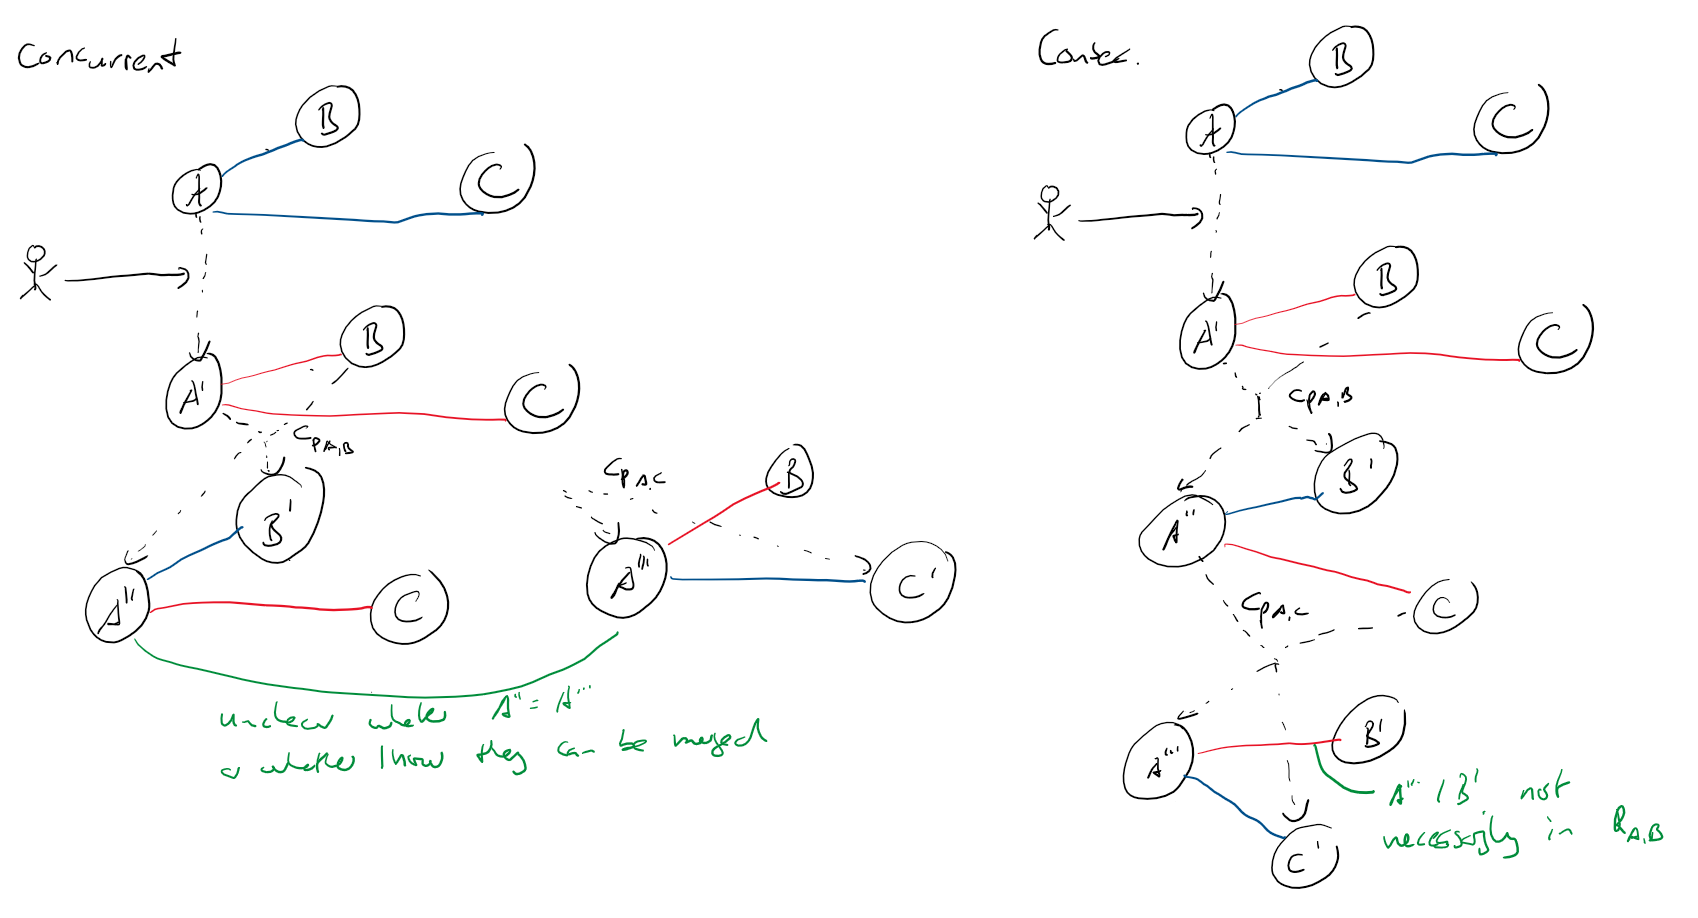
\includegraphics[width=\textwidth]{figures/correctness/formal/concurrent_consecutive_execution.png}
    \caption{Scenarios for independently executing consistency preservation rules on input models and consecutively executing them on the results of other rules.}
    \label{fig:correctness:concurrent_consecutive_execution}
\end{figure}

\mnote{Unification and orchestration necessary due to conflicting sequences}
The examples for the two strategies of executing \glspl{consistency preservation rule} are depicted in \autoref{fig:correctness:concurrent_consecutive_execution}. 
Even if \glspl{consistency preservation rule} were supposed to only modify one model instead of two, like in the examples, the same problems of unification and orchestration would occur as soon as there are two sequences of \glspl{consistency preservation rule} that change the same models.

\mnote{Benefits of consecutive execution}
In our work, we follow the approach of orchestrating and consecutively executing \glspl{consistency preservation rule}.
The benefits of this approach are twofold. First, there is no additional logic required for unifying the changes performed by independently executed \glspl{consistency preservation rule}. 
Second, the unification may deliver a model that is not consistent to any of the \glspl{consistency relation} anymore, whereas consecutive execution at least gives the guarantee that the models are consistent to the last applied \gls{consistency preservation rule}.
With this approach, the preservation rules can \enquote{negotiate} a solution by reacting to the changes the others performed.

\begin{remark} 
\mnote{Monolithic notions are degraded modular ones}
Finally, every monolithic notion of consistency and its preservation can be considered a special case of a modular notion. Having only one consistency relation and one function that preserves it degrades the problem by making the necessity to perform an orchestration of functions obsolete.
\end{remark}

\mnote{Different realization options for consistency preservation rules}
For now, the introduced \glspl{consistency preservation rule} can be any kind of functions that return consistent models. 
Their realization may, for example, be transformations that define how to react to certain changes for restoring consistency, or constraint solvers that find consistent models by solving consistency constraints. 
We do not yet need to consider how these functions are realized to derive consistent models, although, later, we will focus on transformation-based approaches.


\subsection{Declarative and Imperative Consistency Specifications}

\begin{figure}
    \centering
    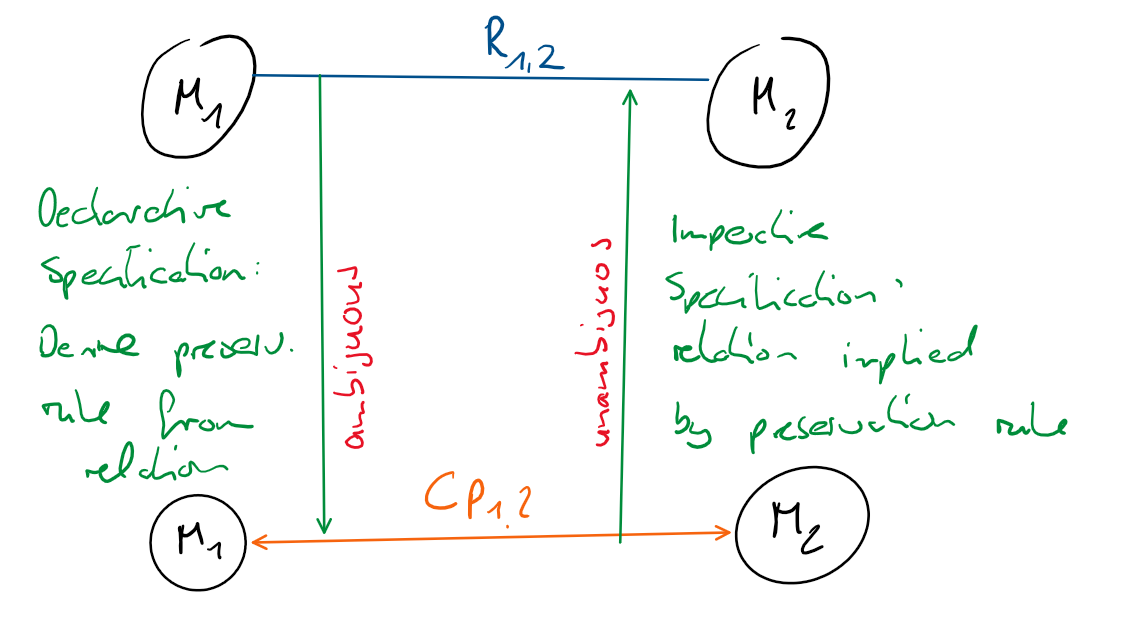
\includegraphics[width=0.7\textwidth]{figures/correctness/formal/declarative_imperative}
    \caption{Declarative and imperative specification of consistency relations and consistency preservation rules}
    \label{fig:correctness:declarative_imperative}
\end{figure}

\mnote{Only define relation \emph{or} function}
We discussed that consistency preservation can be considered as functions, called \glspl{consistency preservation rule}, that preserve consistency according to some relations.
%In practice, consistency preservation is usually specified by means of transformations.
In practice, however, one will usually not specify both the \gls{consistency relation} itself and also the \gls{consistency preservation rule} that preserves it.
Instead, usually one artifact is given and the other is implied or derived.
This leads to the two approaches of \emph{declarative} and \emph{imperative} consistency specifications, depending on whether the specification defines \emph{how} consistency is achieved.
The relation between the two approaches and \glspl{consistency relation} and \glspl{consistency preservation rule} is depicted in \autoref{fig:correctness:declarative_imperative}.

\mnote{Ambiguity in deriving rules from relations}
As a first option, a developer may only define relations that specifies consistency. Functions that preserve these relations can be derived from that.
This is called a \emph{declarative} specification, because it only declares when models are consistent but \emph{how} consistency is achieved.
In general, there is not only a single option how this function can look like.
It can, for example, calculate the result with minimal differences to the input, according to some defined metrics.
Or, especially if there is an intensional specification of that relation, the approach may consider the type of input change and calculate an appropriate change according to the constraints in the intensional specification.
This is the approach that is followed by many declarative transformation languages, such as \gls{QVTR}, or \glspl{TGG}.

\mnote{Relations are induced by fixed-points of functions}
As a second option, a developer can define \glspl{consistency preservation rule}.
These functions imply the underlying \glspl{consistency relation} that they preserve.
Given a function $\function{Cp}$, the relation is implied by its fixed-points: $\consistencyrelation{R}{} = \setted{\modelset{m} \mid \function{Cp}(\modelset{m}) = \modelset{m}}$.
If a function preserving consistency does not perform any changes, the models are, by definition, consistent.
This is called a \emph{imperative} specification, because it declares \emph{how} consistency can be achieved.
Such an approach is followed by many imperative transformation languages, such as \gls{QVTO} or \gls{VIATRA}.


\subsection{Artifacts in Consistency Preservation}

\mnote{Four artifacts for general consistency preservation}
We have discussed that consistency can be considered in a monolithic or modular way. We have, however, also mentioned that the monolithic case can be considered as a special case of the modular one.
For the general case, we thus know from the previous considerations that in a consistency preservation process at least specification that define consistency, called \emph{\glspl{consistency relation}}, functions that preserve consistency, called \emph{\glspl{consistency preservation rule}}, and a function for orchestrating the functions, in the following called \emph{\gls{orchestration function}}, are necessary. Finally, we also need a function that applies the \glspl{consistency preservation rule} in the order that is determined by the orchestration function, which we call the \emph{\gls{application function}}.
To summarize, we consider the following artifacts necessary to handle consistency preservation:
\begin{properdescription}
    \item[\Glspl{consistency relation}:] Binary (or in general n-ary) relations that specify when models are to be considered consistent.
    \item[\Glspl{consistency preservation rule}:] Functions that that restore consistency for a pair (or in general set) of models after they were modified to an inconsistent state.
    \item[\Gls{orchestration function}:] A function that determined in which order the consistency preservation rules have to be executed when the models became inconsistent.
    \item[\Gls{application function}:] A function that is able to apply the consistency preservation rules in the order determined by the orchestration function. 
\end{properdescription}

\mnote{Distinction between orchestration and application}
We explicitly distinguish the orchestration and the application to be able to make more fine-grained statements about the responsibilities for the orchestration and its actual execution.
The process is depicted in \autoref{fig:formal:executionprocess}. Given models that are consistent according to some consistency relations and changes to them that lead to inconsistencies, the orchestration function delivers an order of consistency preservation rules, which is used to parametrize the application function that executes these rules in the given order.
The result is, in the best case, a set of models that is consistent to the relations again.
However, we will see that this is not always possible. Thus, we will especially discuss relevant properties of the artifacts, such as correctness and optimality that reflect how and when this process can be executed successfully.

\begin{figure}
    \centering
    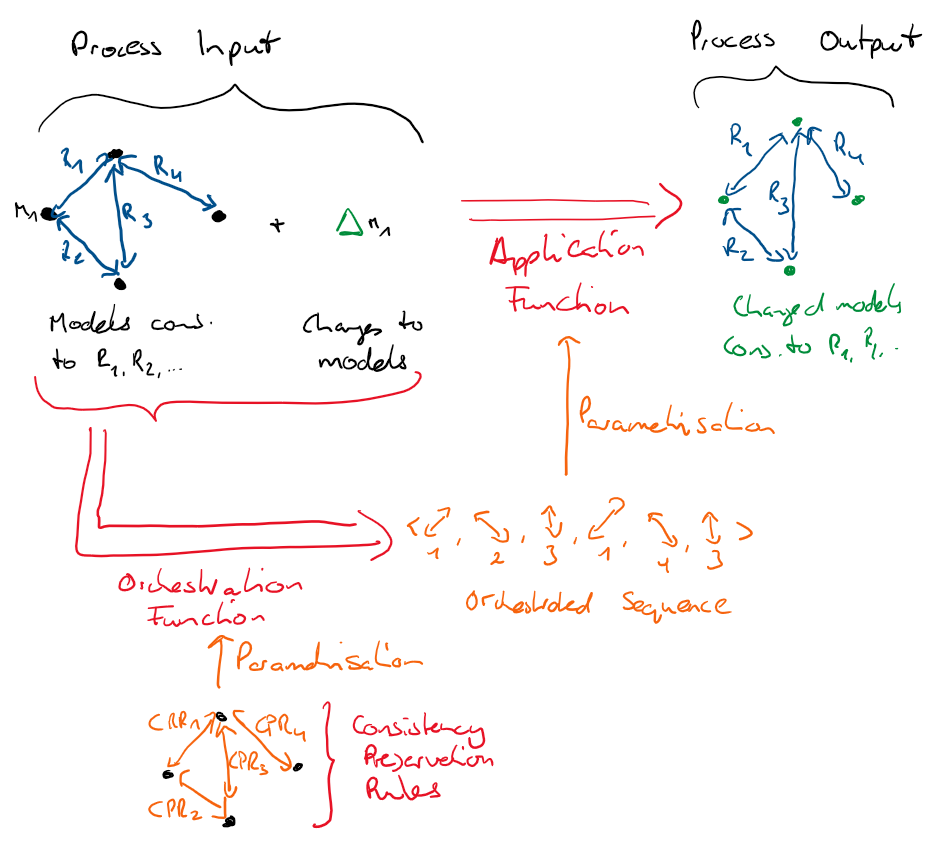
\includegraphics[width=\textwidth]{figures/correctness/formal/execution_process.png}
    \caption{Execution process and artifacts for a modular consistency specification}
    \label{fig:formal:executionprocess}
\end{figure}



%%
%% CORRECTNESS NOTIONS
%%
\section{Notions of Correctness for Consistency Specifications}

%\todo{Define correctness based on a networks adhering to the behavior of a multidirectional transformation}

%\todo{Korrektheit bx Netzwerk: es gib mx, deren Verhalten die bx emulieren müssen. Ist sehr stark, daher abschwächen. Ds muss nur kons. Zustand erreicht werden, egal wie? Einschränkung das original delta nicht geändert wird ist auch für mx künstlich.}

%\todo{Modular implies monolithic -> implicit correctness definition by implied relations}

\mnote{Different notions of correctness}
Before we formally define the above introduced artifacts, such as \glspl{consistency relation}, \glspl{consistency preservation rule}, an \gls{orchestration function} and an \gls{application function}, we first discuss different notions of \emph{correctness} for them.
Since there are different dimensions of correctness, we need to clarify which of them is relevant for us and will be defined in the formalization.

% \begin{definition}[Monolithic \ModelLevelConsistencyPreservationRule]
%     Given two metamodels $\metamodeltuple{M} = \tupled{\metamodelsequence{M}{n}}$ and a \modellevelconsistencyrelation between them $\consistencyrelation{CR}{} \subseteq \metamodelinstanceset{M}{1} \times \dots \times \metamodelinstanceset{M}{n}$.
%     A \emph{monolithic \modellevelconsistencypreservationrule} is a function:
%     \begin{align*}
%         \consistencypreservationrule{\consistencyrelation{CR}{}} : (\metamodeltupleinstanceset{M}, \metamodelinstanceset{M}{2}, \change{\metamodel{M}{1}}) \rightarrow \change{\metamodel{M}{2}}
%     \end{align*}
%     It that takes two consistent models and a change in the first one and returns a change in the second one.
%     We call a \modellevelconsistencypreservationrule \emph{correct} w.r.t. $\consistencyrelation{CR}{}$ if the resulting models when applying the input and output change are consistent to $\consistencyrelation{CR}{}$ again:
%     \begin{align*}
%         &
%         \forall \model{m}{1} \in \metamodelinstanceset{M}{1}, \model{m}{2} \in \metamodelinstanceset{M}{2} :
%         \tupled{\model{m}{1}, \model{m}{2}} \in \consistencyrelation{CR}{} \Rightarrow\\
%         & \formulaskip
%         \forall \change{\metamodel{M}{1}} \in \changeuniverse{\metamodel{M}{1}} :
%         \exists \change{\metamodel{M}{2}} \in \changeuniverse{\metamodel{M}{2}} :\\
%         & \formulaskip
%         \consistencypreservationrule{\consistencyrelation{CR}{}}(\model{m}{1}, \model{m}{2}, \change{\metamodel{M}{1}}) = \change{\metamodel{M}{2}} 
%         \land \tupled{\change{\metamodel{M}{1}}(\model{m}{1}), \change{\metamodel{M}{2}}(\model{m}{2})} \in \consistencyrelation{CR}{}
%     \end{align*}
% \end{definition}


\subsection{Relative Correctness Notions}

\mnote{Intuitive notion of correctness}
The overall objective regarding correctness of consistency preservation is to find models that are actually consistent.
Intuitively speaking, artifacts are correct if they fulfill their intended purpose. 
In our case this means, that consistency relations should consider models consistent whenever they are actually supposed to be considered consistent. 
\Glspl{consistency preservation rule} should return models that are actually consistent according to a \gls{consistency relation} to be considered correct.
This also conforms to the notion of correctness for transformations, which represent \glspl{consistency preservation rule}, defined by \textcite{stevens2010sosym}.
And finally, the orchestration and application functions should execute the \glspl{consistency preservation rule} such that all models are consistent according to all relations afterwards.

\mnote{Correctness is relative}
Correctness of an artifact is always considered with respect to some other specification, be it formally defined or only an informal notion.
For example, consistency relations may be supposed to be correct with respect to some informal notion of correctness that is collected by domain experts and requirements engineers.
A \gls{consistency preservation rule} should always be consistent with respect to a consistency relation. As discussed before, this relation may either be defined explicitly and the preservation rule has to be correct with respect to it, or it may be induced by the fixed points of the preservation rule.
In the latter case, the \gls{consistency preservation rule} will always be correct by construction.


\subsection{Correctness regarding Global Knowledge}

\mnote{Correctness of modular w.r.t. monolithic specification}
We previously distinguished between monolithic and modular notions of consistency.
In the above considerations, we relate the artifacts of a modular (or in the special case also a monolithic) specification to each other.
Another notion of correct, however, can also be defined by relating a modular artifact to a corresponding monolithic artifact.
For example, a set of modular \glspl{consistency relation} may be considered correct with respect to a monolithic relation when it considers the same sets of models consistent.
For three metamodels $\metamodel{M}{1}, \metamodel{M}{2}, \metamodel{M}{3}$ with three modular consistency relations $\consistencyrelation{R}{1,2}, \consistencyrelation{R}{1,3}, \consistencyrelation{R}{2,3}$ between them, as well as a ternary consistency relation $\consistencyrelation{R}{1,2,3}$, we could say that $\consistencyrelation{R}{1,2}, \consistencyrelation{R}{1,3}, \consistencyrelation{R}{2,3}$ are correct (with respect to $\consistencyrelation{R}{1,2,3}$) if and only if:
\begin{align*}
    & \forall \model{m}{1} \in \metamodel{M}{1}, \model{m}{2} \in \metamodel{M}{2}, \model{m}{3} \in \metamodel{M}{3}: \tupled{\model{m}{1}, \model{m}{2}, \model{m}{3}} \in \consistencyrelation{R}{1,2,3} \\
    & \formulaskip
    \equivalent \tupled{\model{m}{1}, \model{m}{2}} \in \consistencyrelation{R}{1,2} \land \tupled{\model{m}{1}, \model{m}{3}} \in \consistencyrelation{R}{1,3} \land \tupled{\model{m}{2}, \model{m}{3}} \in \consistencyrelation{R}{2,3}
\end{align*}
%
We may, analogously, define correctness for \glspl{consistency preservation rule}, an \gls{orchestration function}, and an \gls{application function} with respect to a single monolithic \gls{consistency preservation rule} by defining that both deliver the same results for the same inputs or at least return a consistent result in the same cases.

\begin{figure}
    \centering
    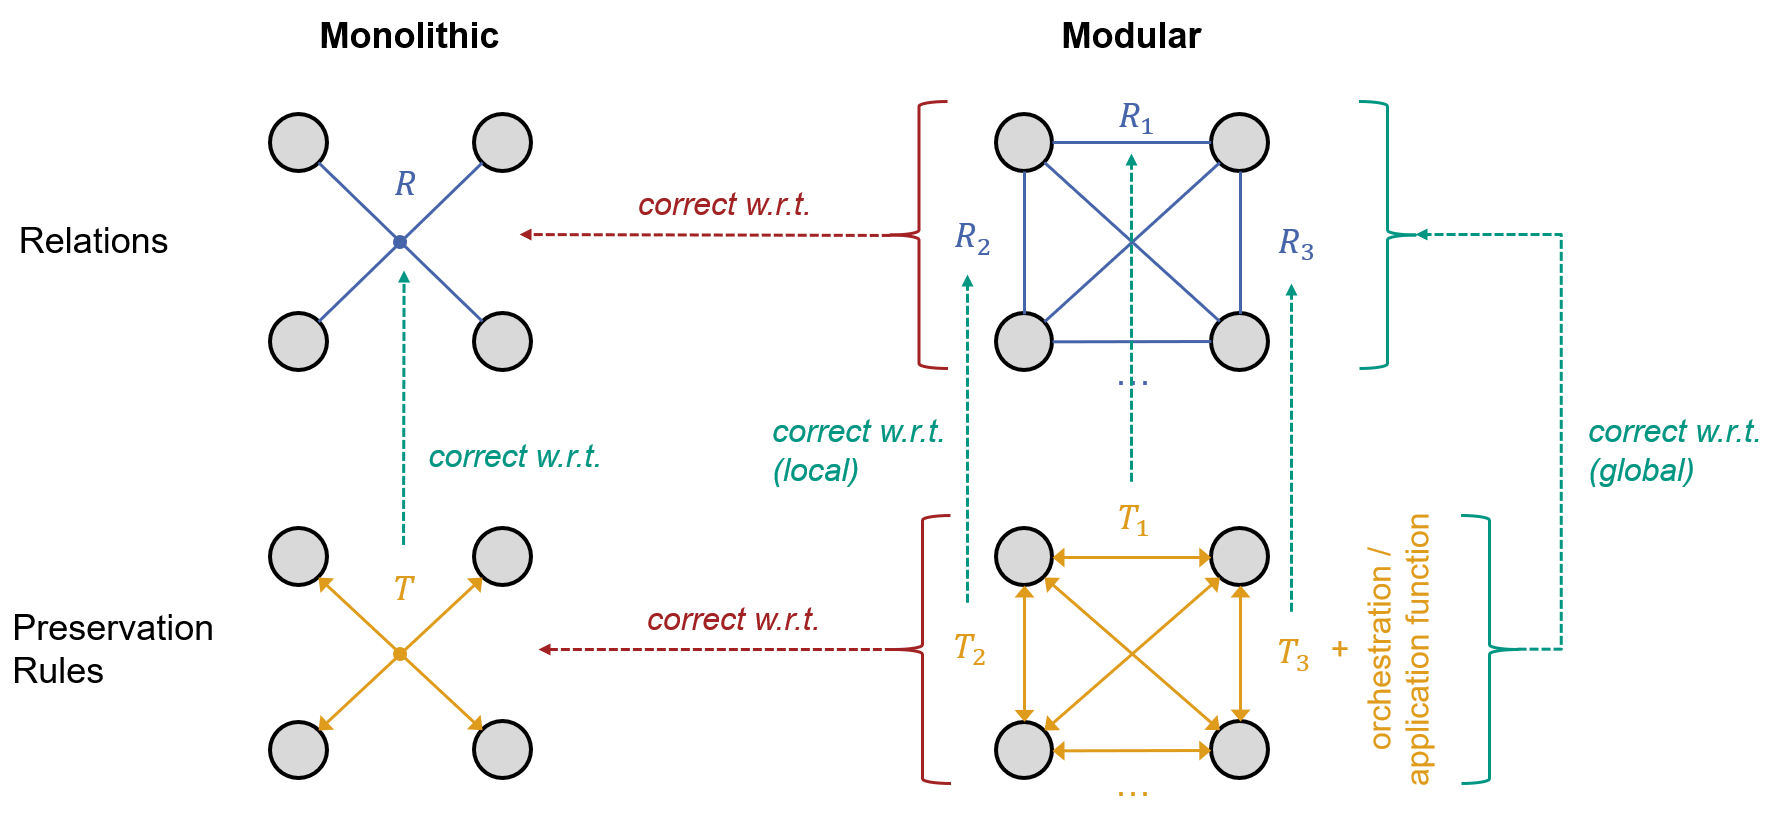
\includegraphics[width=\textwidth]{figures/correctness/formal/correctness_notions.png}
    \caption{Different notions of correctness for consistency and its preservation}
    \label{fig:correctness:correctnessnotions}
\end{figure}


\subsection{Dimensions of Correctness}

\mnote{Two dimension of correctness notions}
The discussed correctness notions introduce two dimension: First, correctness can be considered between artifacts within a monolithic or modular specification. Second, correctness can be considered between artifacts of a modular specification and corresponding artifacts of a monolithic specification. These dimension and correctness relations are depicted in \autoref{fig:correctness:correctnessnotions}.
The former dimension is depicted vertically. \Glspl{consistency preservation rule} need to be correct with respect to their \glspl{consistency relation}.
In the modular case, in addition to each preservation rule being \emph{locally} correct with respect to its relation, the combination of preservation rules by means of an orchestration and application function must also be correct with respect to the combination of all relations.
The latter dimension is depicted horizontally. Each modular artifact is supposed to be consistent with respect to its corresponding monolithic artifact.

\mnote{Drawbacks of global specification notions}
Although correctness of modular with respect to monolithic artifacts can be interesting from a theoretical perspective, its practical relevance is limited.
That notion of correctness assumes that there is some kind of global truth that has to be reflected by a modular specification.
This, however, has two essential drawbacks:
\begin{description}
    \item[Validation Artifacts:] The artifacts to check correctness against, i.e., the global, monolithic \gls{consistency relation} as well as an appropriate monolithic \gls{consistency preservation rule}, do usually not exist. If they existed, they could directly be used to preserve consistency. Thus, it is impossible to validate a set of \glspl{consistency relation} and \glspl{consistency preservation rule} against such a global specification.
    \item[Modular Knowledge:] This notion of correctness requires that the developers have some global knowledge that represents a monolithic \gls{consistency relation} and its \gls{consistency preservation rule}. As discussed before, we assume  the knowledge about relations between models to usually be distributed across several persons. Thus, there will no be such global knowledge, thus not even an implicit notion of the necessary artifacts to validate the modular specifications against. not to be mention an explicit representation.
\end{description}
%
Since this conflicts with our assumption of distributed knowledge about relations and independently developed, modular specification, we do not further consider this notion of consistency.
In this thesis, we focus on correctness between the artifacts of a modular consistency specification.


\subsection{Correctness of Consistency Relations}

\mnote{Correctness of relations}
The consistency notion that we consider in the following especially requires that \glspl{consistency preservation rule} and the functions to orchestrate and apply them must be correct with respect to \glspl{consistency relation}.
This notion, however, does not define when \glspl{consistency relation} are considered \emph{correct}.
One option is to only consider correctness with respect to monolithic artifacts for the case of \glspl{consistency relation}, as we proposed in previous work~\cite{klare2019icmt}.
This, however, suffers from the drawbacks discussed before, requiring a global notion of consistency.
Another notion of correctness would be conformance of the specified relations with what developers expect to be consistent, i.e., a validation of requirements.
For example, a consistency relation between UML and Java may only be considered correct if it fulfills some \enquote{natural} notion of consistency, as people know how elements have to be related because they represent similar things, such as classes, or because a standard like the UML~\cite{uml} prescribes that.
In this work, however, we do not consider such a correctness notion with respect to external, maybe not formally specified artifacts, which is part of separate research on requirements engineering and validation.

\mnote{Relations are not correct by construction}
In consequence, we might say that \glspl{consistency relation} are simply \emph{correct by construction}.
Thus, relations would normatively define what is to be considered consistent.
However, a consequence of not assuming a global knowledge of consistency is that different domain experts may have different notions of when models are to be considered consistent.
Consider for three metamodel $\metamodel{M}{1}, \metamodel{M}{2}, \metamodel{M}{3}$ the three modular \glspl{consistency relation} $\consistencyrelation{R}{1,2} = \setted{\tupled{\model{m}{1},\model{m}{2}}}, \consistencyrelation{R}{1,3} = \setted{\tupled{\model{m}{1},\model{m}{3}}}, \consistencyrelation{R}{2,3} = \setted{\tupled{\model{m}{1},\model{m'}{3}}}$. 
Then there is no triple of models that is considered consistent to all relations. 
Although we still do not want to assume a global knowledge about consistency to which the modular one must conform, we might say that these relations are \emph{incompatible}, as we do not want to combine relations that induce an empty set of consistent model tuples.
Identifying an appropriate notion of \emph{compatibility} and how to check it constitutes \ref{rq:correctness:compatibility} and will be discussed in \autoref{sec:correctness:compatibility}.
%\researchquestion{2.1}{When should independently defined \glspl{consistency relation} be considered \emph{compatible} and how can that compatibility be checked?}

\mnote{Modular relations induce monolithic ones}
In fact, every set of modular \glspl{consistency relation} induces a monolithic one.
This monolithic relation $\consistencyrelation{R}{}$ for metamodels $\metamodelsequence{M}{n}$ and pairwise consistency relations $\consistencyrelation{R}{i,j}$ is defined by:
\begin{align*}
    \consistencyrelation{R}{} = \setted{\tupled{\model{m}{1}, \dots, \model{m}{n}} \mid \bigwedge\limits_{1 \le i < j \le n} \tupled{\model{m}{i}, \model{m}{j}} \in \consistencyrelation{R}{i,j}}
\end{align*}
At least if this induced relation if empty, we probably want to consider the modular relations incompatible, because if no models are considered consistent, we cannot describe any system consistently.


% Keeping multiple models consistent by means of transformations imposes either a single multidirectional transformation or a combination of several bi- or multidirectional transformations.
% Each of these transformations is able to take a consistent tuple of models and a change to them and to return a new consistent tuple of models.

% \mnote{Correctness implicitly covered by definitions}
% \textcite{stevens2010sosym} proposes an explicit notion of \emph{correctness} for transformations. This is based on the fact that her definition of a transformation does only specify that for two given model, which may be inconsistent because one was modified, an update of the other model is returned.
% The requirement that the originally modified model and the one returned by the transformation have to conform to some consistency relations is specified externally as a notion of \emph{correctness}.
% We directly relate a consistency preservation rule that restores consistency to an according consistency relation, thus a consistency preservation rule that follows our definition is correct by construction in terms of the correctness definition by \citeauthor{stevens2010sosym}.
% The same applies to the consistency preservation application function, which we consider \emph{correct} if it fulfills its definition, as that definition already covers all requirements to that function.

% \mnote{Different notions of correctness}
% In general, correctness can be considered in two ways: First, an artifact may be correct if it simply follows its definition.
% While for consistency relations, changes and the generic \modellevelconsistencypreservationrule generalization function correctness can be canonically achieved, this is not that simple for a consistency preservation rule and the consistency preservation application function, as they have to fulfill some constraints with respect to consistency relations they rely on.
% Second, an artifact may be correct if it fulfills some, maybe only implicitly known specification. For example, a consistency relation between UML and Java may only be considered correct if it fulfills some \enquote{natural} notion of consistency, as people know how elements have to be related because they represent similar things, such as classes, or because a standard like the UML~\cite{uml} prescribes that.

% \mnote{Correctness regarding global specifications}
% In this work we do not consider the latter correctness notion with respect to external, maybe not formally specified artifacts, which is part of separate research on validation.
% However, when considering consistency of multiple models it may be standing to reason that a modular specification of consistency and its preservation has to be correct with regards to some global, monolithic specification. More precisely, there may be a multiary relation putting several metamodels into relation, which the developers at least implicitly know, and a set of binary relations somehow has to respect that multiary relation, i.e., be \emph{correct} with respect to that relation.
% The same can be imagines for consistency preservation. One may define a multidirectional transformation for a multiary relation, taking a tuple of changes to consistent models and retuning a new tuple of changes, which applied to the models delivers a consistent set of models again. In fact, this would be a realization of the behavior of the consistency preservation application function without relying on modular \modellevelconsistencypreservationrules.

% \begin{description}
%     \item[Validation Artifacts:] The artifacts to check correctness against, i.e., the global, multiary consistency relation as well as an appropriate multidirectional transformation, do usually not exist. If they existed, they could directly be used to preserve consistency. Thus is impossible to validate a set of consistency relations and preservation rules against such a global specification.
%     \item[Modular Knowledge:] This notion of correctness requires that the developers have some global knowledge that represents a monolithic, multiary consistency relation and their preservation rules. Usually, this will not be the case, so there is even no implicit notion of the necessary artifacts to validate the modular specifications against, not to be mention an explicit representation.
% \end{description}

%\todo{Add an image for that relation}

% Overall Goals:
% \begin{itemize}
%     \item Define correctness of a transformation network: termination in consistent state
% \end{itemize}



%%
%% FORMALIZATION
%%
\section{A Formal Notion of Transformation Networks}

\mnote{Goal: formalize transformation networks and correctness notions}
We yet discussed a general notion of consistency and its preservation with a focus on a modular way of specifying it.
This notion, however, was only specified in a rather informal way to first be able to discuss correctness notions and determine which notion is relevant for the considerations in this thesis.
In the following, we define a formal notion of consistency and its preservation, based on the informal explanation given before.
We also give a precise definition of notions for correctness between the artifacts of a modular specification.
Furthermore, we now focus on transformation-based approaches for preserving consistency, i.e., we consider specifications that transform changes within one or more models into changes in one or more other models.

Allgemeine Definition Transformationsnetzwerke:
\begin{itemize}
    %\item Definition Transformation aus Relation und Wiederherstellungsroutinen; Routinen nehmen n Modelle und n Deltasequenzen (eine pro Modell) und liefern n Deltasequenzen zurück.
    %\item Im Allgemeinen könnte eine Transformation beliebige dieser Deltasequenzen modifizieren. Wir verlangen jedoch, dass eine Transformation nur Deltas anhängt, also die Sequenzen länger werden
    %\item Genauer beschränken wir auch, welche Sequenzen eine Transformation sehen und ändern darf, genau gesagt darf sie die Sequenzen von zwei Modellen sehen und eine davon verlängern.
    \item Hier kommt bereits der Unterschied zu bisherigen Transformationen, denn die sehen nur Deltas an einem Modell und erzeugen Deltas an dem anderen. Das ist bei uns schon gänzlich anders. Bidirektionale Transformationen unterstützen das im Übrigen auch nicht, sondern sind nur Spezifikationen, aus denen sich Wiederherstellungsroutinen für beide Richtungen ableiten lassen (siehe Stevens 2010)
    %\item Relationen in erster Instanz auf Modellebene (also bzgl. ganzer Modelle, nicht einzelner Modellelemente) definieren
    %\item Direkt als multidirektionale Transformation definieren, also beliebig viele geändert Ein- und Ausgabemodelle (oder jeweils nur eins?)
    %\item Korrektheit einer Transformation (nach Stevens) definieren!
    \item Versuchen den Konkatenationsoperator zu definieren ohne dass er alle Metamodelle referenzieren muss (also Transformation wählt aus einer großen Eingabemenge relevanten Modelle aus, ändert relevante und dann fügt der Operator sie in die große Menge ein)
    \item Definition Transformationsnetzwerk als Tupel aus Metamodellen, Transformationen und einer Ausführungsfunktion. 
    \item Die Ausführungsfunktion führt für eine gegebene Änderung eine Auswahl der Transformationen nacheinander aus.
    \item Korrektheit eines Netzwerkes definieren: Die Ausführungsfunktion erzeugt eine Transformationssequenz, die angewendet auf eine Änderung für alle Änderungen ein korrektes Ergebnisse produziert, d.h. die Modelle sind konsistent bzgl. allen Konsistenzrelationen.
\end{itemize}


\subsection{Modular Consistency Specification}

\mnote{Extensional specifications are relations}
As already discussed informally before, an extensional specification of consistency enumerates all sets of models that are considered consistent to each other, i.e., it specifies a relation between the models.
Since it eases comprehension of the definitions if the considered models are identifiable with an index, we will consider, without loss of generality, tuples rather than sets of models throughout the rest of this thesis.

\begin{definition}[\ModelLevelConsistencyRelation]
    Given a tuple of metamodels $\metamodeltuple{M} = \tupled{\metamodelsequence{M}{n}}$, a \emph{\modellevelconsistencyrelation} $\consistencyrelation{CR}{}$ is a relation for instances of the metamodels $\consistencyrelation{CR}{} \subseteq \metamodeltupleinstanceset{M} = \metamodelinstanceset{M}{1} \times \dots \times \metamodelinstanceset{M}{n}$.

    For a tuple of models $\modeltuple{m} = \tupled{\model{m}{1}, \dots, \model{m}{n}} \in \metamodeltupleinstanceset{M}$ we say that:
    \begin{align*}
        \modeltuple{m} \consistenttomath \consistencyrelation{CR}{} \equivalentperdefinition \modeltuple{m} \in \consistencyrelation{CR}{}
    \end{align*}
    Otherwise, we call $\modeltuple{m} \mathtext{inconsistent to} \consistencyrelation{CR}{}$.
\end{definition}

\mnote{Start with coarse-grained model-level relations}
Given a tuple of models, we consider that tuple of models consistent if it is contained in the consistency relation.
This conforms to consistency definitions such as the one proposed by \textcite{stevens2010sosym} for bidirectional transformations.
We explicitly denote this kind of consistency relation as \emph{model-level}, because we will later need a more fine-grained notion of consistency relations at the level of \metaclasses and need to distinguish between the two.

\mnote{Modular notions of consistency}
If a single relation describes consistency between all relevant models, consistency is directly defined by means of model tuples being in that relations. We call such a relation a \emph{monolithic relation}.
However, if we have a \emph{modular} notion of consistency, i.e., a relation does only define consistency between some of the relevant models and the global notion of consistency is defined by a combination of several such relations, we need an explicit definition for that notion.
For the sake of simplicity, we focus on binary relations as a modular representation of consistency, but this definition could also be generalized to relations of arbitrary arity.
We assume that there is only one consistency relation between each pair of metamodels.
This assumption is without loss of generality, because two relations between the same metamodels are equivalent to only considering their intersection, i.e., only the model pairs that are considered consistent by both relations.

\todo{wlog: no direction of relation}

\begin{definition}[Consistency]
    Let $\metamodeltuple{M} =  \tupled{\metamodelsequence{M}{n}}$ be metamodels and let $\consistencyrelation{CR}{i,j} \subseteq \metamodelinstanceset{M}{i} \times \metamodelinstanceset{M}{j}$ be a binary \modellevelconsistencyrelation for any two metamodels $\metamodel{M}{i}, \metamodel{M}{j} \in \setted{\metamodelsequence{M}{n}}$.
    For a given tuple of models $\modeltuple{m} = \tupled{\model{m}{1}, \dots, \model{m}{n}} \in \metamodeltupleinstanceset{M}{} = \metamodelinstanceset{M}{1} \times \dots \times \metamodelinstanceset{M}{n}$, we say that this model tuple is \emph{consistent to} $\consistencyrelation{CR}{i,j}$ if and only if the instances of $\metamodel{M}{i}$ and $\metamodel{M}{j}$ are in that relation:
    \begin{align*} 
        &
        \modeltuple{m} = \tupled{\model{m}{1}, \dots, \model{m}{n}} \consistenttomath \consistencyrelation{CR}{i,j} \equivalentperdefinition %\\
        %& \formulaskip
        \tupled{\model{m}{i},\model{m}{j}} \in \consistencyrelation{CR}{i,j}
        %\exists \model{m}{i} \in \metamodelinstanceset{M}{i}, \model{m}{j} \in \metamodelinstanceset{M}{j} : \model{m}{i} \in \modelset{m} \land \model{m}{j} \in \modelset{m} \land \tupled{\model{m}{i}, \model{m}{j}} \in \consistencyrelation{CR}{}
    \end{align*}
    For a set of binary \modellevelconsistencyrelations $\consistencyrelationset{CR}$ for metamodels $\metamodeltuple{M}$, we say that a tuple of models $\modeltuple{m} \in \metamodeltupleinstanceset{M}{}$ is \emph{consistent to} $\consistencyrelationset{CR}$ if and only if it is consistent to each consistency relation in that set:
    \begin{align*} 
        &
        \modeltuple{m} \consistenttomath \consistencyrelationset{CR} \equivalentperdefinition %\\
        %& \formulaskip
        \forall \consistencyrelation{CR}{} \in \consistencyrelationset{CR} : \modeltuple{m} \consistenttomath \consistencyrelationset{CR}
    \end{align*}
\end{definition}

\mnote{Examplary binary relations}
The definition states that given a set of \modellevelconsistencyrelations the models must be consistent to all of these relations to consider them consistent to the set.
Consider, for example, the relations $\consistencyrelation{CR}{1} = \setted{\tupled{\model{m}{1}, \model{m}{2}}}$, $\consistencyrelation{CR}{2} = \setted{\tupled{\model{m}{2},\model{m}{3}}}$, $\consistencyrelation{CR}{3} = \setted{\tupled{\model{m}{1}, \model{m}{3}}}$ with $\model{m}{i} \in \metamodelinstanceset{M}{i}$ for metamodels $\metamodel{M}{i}$. Then the model tuple $\tupled{\model{m}{1}, \model{m}{2}, \model{m}{3}}$ is consistent to these relations, because it is consistent to each of the binary relations.
These consistency relations are equivalent to a monolithic relation $\consistencyrelation{CR}{} = \setted{\tupled{\model{m}{1}, \model{m}{2}, \model{m}{3}}}$, because a model tuple $\modeltuple{m}$ is consistent to $\consistencyrelation{CR}{}$ exactly when it is consistent to $\setted{\consistencyrelation{CR}{1}, \consistencyrelation{CR}{2}, \consistencyrelation{CR}{3}}$.


\subsection{Expressiveness of Modular Consistency Specifications}

\mnote{Modular and monolithic specification are not equivalent}
Although in that exemplary case the binary relations are equivalent to a monolithic relation, such an equivalence is not always given. In general, two interesting insights come along with that definition of consistency based on modular relations. First, expressiveness of defining consistency modularly by a set of relations is not equivalent to defining one monolithic relation between all models. Second, a modular definition of consistency can easily contain contradictions, which may lead to an empty set of consistent models.

\mnote{Binary relations reduce expressiveness}
It is easy to see that a combination of binary relations is not able to express the same consistency relations as one monolithic relation.
For example, the monolithic relation $\consistencyrelation{CR}{} = \setted{\tupled{\model{m}{1}, \model{m}{2}, \model{m}{3}'}, \tupled{\model{m}{1}, \model{m}{2}', \model{m}{3}}, \tupled{\model{m}{1}', \model{m}{2}, \model{m}{3}}}$ cannot be expressed by binary relations.
The binary relations necessarily need to contain $\tupled{\model{m}{1}, \model{m}{2}}$, because $\tupled{\model{m}{1}, \model{m}{2}, \model{m}{3}'} \in \consistencyrelation{CR}{}$ and $\tupled{\model{m}{2}, \model{m}{3}}$, because $\tupled{\model{m}{1}', \model{m}{2}, \model{m}{3}} \in \consistencyrelation{CR}{}$. However, this would mean that $\tupled{\model{m}{1}, \model{m}{2}, \model{m}{3}}$ is considered consistent to the binary relations although it not consistent to the modular relation $\consistencyrelation{CR}{}$.
Thus, using sets of binary relations in contrast to a single monolithic relation reduces expressiveness.
\textcite{stevens2017a} discusses the property of a multiary relation to be expressed by binary ones as \emph{binary-definable} in detail.
She proposed restrictions to binary relations that may be sufficient and still practical for expressing consistency, such as a notion of \emph{binary-implemented} relations.
However, we reasoned the assumption that relations need to be specified independently and thus modularly anyway, thus we have to accept that these restrictions in expressiveness exists.
\todo{visualize}

\mnote{Binary relations may be contradictory}
Additionally, it is easy to define multiple binary relations of which each can be fulfilled by certain models, but for which no tuple of models exists that is consistent to all of them. Consider the relations $\consistencyrelation{CR}{1} = \setted{\tupled{\model{m}{1}, \model{m}{2}}}$, $\consistencyrelation{CR}{2} = \setted{\tupled{\model{m}{2}, \model{m}{3}}}$, $\consistencyrelation{CR}{3} = \setted{\tupled{\model{m}{1}, \model{m}{3}'}}$.
Although for each of these relations a consistent set of models exists, which is exactly the one defined in each relation, no tuple of models exists that fulfills their combination.
This example already demonstrates the worst case, in which no consistent models exist for a set of relations.
In other cases, it may be possible that only for some models that are consistent according to one or some of the relations no model tuple exists that is consistent for all models.
Consider the relations $\consistencyrelation{CR}{1} = \setted{\tupled{\model{m}{1}, \model{m}{2}}}$, $\consistencyrelation{CR}{2} = \setted{\tupled{\model{m}{2}, \model{m}{3}}, \tupled{\model{m}{2}, \model{m}{3}}'}$, $\consistencyrelation{CR}{3} = \setted{\model{m}{1}, \model{m}{3}'}$.
In this case, the tuple $\tupled{\model{m}{1}, \model{m}{2}, \model{m}{3}'}$ would be considered consistent to the relations, but although $\tupled{\model{m}{2}, \model{m}{3}} \in \consistencyrelation{CR}{2}$ there exists no $\model{m^*}{1} \in \metamodelinstanceset{M}{1}$ so that $\tupled{\model{m^*}{1}, \model{m}{2}, \model{m}{3}}$ is consistent to all these relations.
\todo{visualize}

\mnote{Sets of relations can forbid models}
It is easy to see that one monolithic relation may be equally represented by an arbitrary number of sets of binary relations by simply adding model pairs to these binary relations that are never consistent to the other relations, like we have seen for the pair $\tupled{\model{m}{2}, \model{m}{3}}$ in the previous example.
This means that the combination of relations can lead to the situation that some models are actually forbidden (like $\model{m}{3}$ in the example before) due to the combination of consistency relations.
We already informally discussed this as a notion of \emph{compatibility}, for which we investigate in \autoref{sec:correctness:compatibility} how far this behavior is or should be expected.


\subsection{Incremental and Inductive Consistency Preservation}

\mnote{Preserving consistency}
While the previous discussion only considered when models are considered consistent, it is of especial interest to ensure that consistency of models is preserved.
We informally introduced such specifications as \glspl{consistency preservation rule}.
In the following, we will restrict us to \emph{incremental} and \emph{inductive} consistency preservation and give a precise definition for that.
This means that we make the following assumptions to the process:
\begin{properdescription}
    \item[Information preservation (incrementality):] After a change to one model, the others are not generated from scratch but updated according to the performed changes. This ensures that information that cannot be generated but was added by users to the other models is preserved.
    \item[Consistency assumption (induction):] We assume models to be consistent before a change is processed by \glspl{consistency preservation rule}. Otherwise the preservation rules would need to be able to handle arbitrary states of the models and it would be unclear consistency to which \glspl{consistency relation} has to be restored.
\end{properdescription}
While incrementality is an essential requirement whenever consistency shall be preserved to avoid information loss, inductivity may not be necessary.
We, however, make this assumption to avoid requiring from the \glspl{consistency preservation rule} that they need to be able to process an inconsistent state without knowing which changes introduced it.
From a theoretical point of view, we could omit that requirement, but this would make the specification of \glspl{consistency preservation rule} impractically complicated, such that omitting that requirement is not practically relevant anyway.
%In consequence, an incremental and inductive \gls{consistency preservation rule} takes a consistent tuple of models and changes to them and returns a tuple of models that is consistent again.

\todoLater{Do we need inductivity for synchronization? Otherwise we may remove it here and from following definitions?}
%\todo{Explicitly discuss incrementality here, although we actually do not need it. So leave it out? No, needed for synchronization definition. But make clear that this is a specialization and discuss generalization.}
%\todo{Make precise here that we have incremental consistency, thus last consistent state and delta to that is known. We did not assume that in the informal notion before.}

\mnote{Monolithic and modular consistency preservation}
Like we already discussed for \glspl{consistency preservation rule} in general, incremental preservation rules can be realized in an either monolithic or modular way.
A monolithic consistency preservation rules takes a tuple of models that is consistent to a consistency relation and a change to these models and returns another tuple of models that is consistent again.
In a modular specification of \glspl{consistency preservation rule}, a set of such rules is given which are able to preserve consistency of a subset of the given models according to modular consistency relations.
In our case, we consider such rules for two models, each of them restoring consistency according to a binary consistency relation.
%We will later discuss if and how an execution order of such consistency preservation rules can be determined.

\mnote{Drawbacks of existing unidirectional consistency restorers}
In terminology for transformations, a \gls{consistency preservation rule} that restores consistency of models according to a \gls{consistency relation} in one direction is called \emph{directional transformation}~\cite{stevens2010sosym} or \emph{consistency restorer}~\cite{stevens2020BidirectionalTransformationLargeSoSym}.
Definitions of that terminology do usually not consider changes but only states of models and simply define a preservation rule for metamodel $\metamodel{M}{1}$ and $\metamodel{M}{2}$ that modifies the instance of $\metamodel{M}{2}$ to restore consistency as $\consistencypreservationrule{}: \metamodelinstanceset{M}{1} \times \metamodelinstanceset{M}{2} \rightarrow \metamodelinstanceset{M}{2}$.
This notion, however, has two properties that imply essential drawbacks:
\begin{properdescription}
    \item[State-based:] No information about the performed changes that led to the inconsistent state are given. This means that the specification is not aware of how the inconsistent state was reached.
    \item[Unidirectional:] The unidirectionality of the specification always requires to only update one model to restore consistency.
\end{properdescription}
State-based transformations always suffer from the problem that it is unknown which changes were made that led to an inconsistent state. 
This, for example, includes that information about elements which were moved or renamed can potentially not be reconstructed, leading to elements that are deleted and created anew, losing all information that was potentially added to them \todo{add cite}.
Unidirectionality may be reasonable when assuming that only one of the models was modified. In that case it is sufficient to update the other model to restore consistency.
With a modular specification of consistency preservation, however, several \glspl{consistency preservation rule} modifying the same models may need to be executed.
This can be seen in the example in \autoref{todo}\todo{add graphics and explanation for that}.
In consequence, the rules need to be able to deal with changes performed in both of the input models and, consequentially, need to update both models to reflect the changes in the other.

\mnote{Synchronizing consistency preservation rules circument drawbacks}
To be able to combine several \glspl{consistency preservation rule} without the discussed drawbacks, we define a \emph{synchronizing} rather than a unidirectional notion of them
Those rules are able to react to changes in both models and produce changes in both models again.
To precisely define this behavior, we first introduce a notion of \emph{changes} and afterwards of \emph{\glspl{consistency preservation rule}}.

\begin{definition}[Change]
    Given a metamodel $\metamodel{M}{}$, a change $\change{\metamodel{M}{}}$ is a function that takes an instance of that metamodel and returns another one:
    \begin{align*}
        \change{\metamodel{M}{}}: \metamodelinstanceset{M}{} \rightarrow \metamodelinstanceset{M}{}
    \end{align*}
    It encodes any kind of modification, which may be just an element addition, or removal, an attribute change and so on, or any composition of changes.
    We denote the identity change, i.e., the change that always returns the input model, as $\identitychange$:
    \begin{align*}
        \identitychange(x) \equalsperdefinition x
    \end{align*}
    We denote the universe of all changes in $\metamodel{M}{}$, i.e., all subsets of $\metamodelinstanceset{M}{} \times \metamodelinstanceset{M}{}$ that are functional, as 
    \begin{align*}
        \changeuniverse{\metamodel{M}{}} \equalsperdefinition \setted{\change{\metamodel{M}{}} \mid \change{\metamodel{M}{}} \subseteq \metamodelinstanceset{M}{} \times \metamodelinstanceset{M}{} \land
        (\tupled{\model{m}{1}, \model{m}{2}}, \tupled{\model{m}{1}, \model{m}{3}} \in \change{\metamodel{M}{}} \Rightarrow \model{mc}{2} = \model{m}{3})}
    \end{align*}
    For a given metamodel tuple $\metamodeltuple{M} = \tupled{\metamodelsequence{M}{n}}$, we denote the set of all tuples of changes in the instances tuples of 
    $\metamodeltuple{M}$, i.e. in $\metamodeltupleinstanceset{M}$, as $\changeuniverse{\metamodeltuple{M}}$:
    \begin{align*}
        \changeuniverse{\metamodeltuple{M}} \equalsperdefinition \setted{ \changetuple{\metamodeltuple{M}} = \tupled{\change{\metamodel{M}{1}}, \dots, \change{\metamodel{M}{n}}} \mid \forall i \in \setted{1,\dots,n} : \change{\metamodel{M}{i}} \in \changeuniverse{\metamodel{M}{i}} } 
    \end{align*}
\end{definition}

\mnote{Behavior of unapplicable change is undefined}
For us, it does not matter how the function describing a change behaves in cases, in which the encoded change cannot be applied, e.g., because the changed or removed element does not exist. The function may do nothing for those models, i.e., return the identical model, or even be undefined for those model, i.e., be partial.
\todoLater{Check whether this behavior is correct.}

% \begin{definition}[\ModelLevelConsistencyPreservationRule]
%     Let $\metamodel{M}{1}, \metamodel{M}{2}$ be two metamodels and $\consistencyrelation{CR}{} \subseteq \metamodelinstanceset{M}{1} \times \metamodelinstanceset{M}{2}$ a binary \modellevelconsistencyrelation between them.
%     A \emph{\modellevelconsistencypreservationrule} $\consistencypreservationrule{\consistencyrelation{CR}{}}$ for the relation $\consistencypreservationrule{\consistencyrelation{CR}{}}$ is a function:
%     \begin{align*}
%         \consistencypreservationrule{\consistencyrelation{CR}{}} : (\metamodelinstanceset{M}{1}, \metamodelinstanceset{M}{2}, \change{\metamodel{M}{1}}) \rightarrow \change{\metamodel{M}{2}}
%     \end{align*}
%     It takes two consistent models and a change in the first one and returns a change in the second one.
%     We call a \modellevelconsistencypreservationrule \emph{correct} w.r.t. $\consistencyrelation{CR}{}$ if the resulting models when applying the input and output change are consistent to $\consistencyrelation{CR}{}$ again:
%     \begin{align*}
%         &
%         \forall \model{m}{1} \in \metamodelinstanceset{M}{1}, \model{m}{2} \in \metamodelinstanceset{M}{2} :
%         \tupled{\model{m}{1}, \model{m}{2}} \in \consistencyrelation{CR}{} \Rightarrow\\
%         & \formulaskip
%         \forall \change{\metamodel{M}{1}} \in \changeuniverse{\metamodel{M}{1}} :
%         \exists \change{\metamodel{M}{2}} \in \changeuniverse{\metamodel{M}{2}} :\\
%         & \formulaskip
%         \consistencypreservationrule{\consistencyrelation{CR}{}}(\model{m}{1}, \model{m}{2}, \change{\metamodel{M}{1}}) = \change{\metamodel{M}{2}} 
%         \land \tupled{\change{\metamodel{M}{1}}(\model{m}{1}), \change{\metamodel{M}{2}}(\model{m}{2})} \in \consistencyrelation{CR}{}
%     \end{align*}
% \end{definition}

\begin{definition}[\ModelLevelConsistencyPreservationRule]
    \label{def:consistencypreservationrule}
    Let $\metamodel{M}{1}, \metamodel{M}{2}$ be two metamodels and $\consistencyrelation{CR}{} \subseteq \metamodelinstanceset{M}{1} \times \metamodelinstanceset{M}{2}$ a binary \modellevelconsistencyrelation between them.
    A \emph{\modellevelconsistencypreservationrule} $\consistencypreservationrule{\consistencyrelation{CR}{}}$ for the relation $\consistencypreservationrule{\consistencyrelation{CR}{}}$ is a function:
    \begin{align*}
        \consistencypreservationrule{\consistencyrelation{CR}{}} : (\metamodelinstanceset{M}{1}, \metamodelinstanceset{M}{2}, \changeuniverse{\metamodel{M}{1}}, \changeuniverse{\metamodel{M}{2}}) \rightarrow (\changeuniverse{\metamodel{M}{1}}, \changeuniverse{\metamodel{M}{2}})
    \end{align*}
    %It takes two consistent models and a change in the first one and returns a change in the second one. 
\end{definition}

\mnote{Correctness notion of consistency preservation rules}
To consider a \modellevelconsistencypreservationrule \emph{correct}, it has to return changes that, when applied to the input models, result in models that are consistent according to the \modellevelconsistencyrelation for which the preservation rule is defined.
This conforms to the notion of correctness defined for bidirectional transformations~\cite{stevens2010sosym}.

\begin{definition}[\ModelLevelConsistencyPreservationRule Correctness]
    Let $\consistencypreservationrule{\consistencyrelation{CR}{}}$ be a \emph{\modellevelconsistencypreservationrule}.
    We call a \modellevelconsistencypreservationrule \emph{correct} if the resulting models when applying the generated changes are consistent to $\consistencyrelation{CR}{}$ again:
    \begin{align*}
        &
        \forall 
        \model{m}{1} \in \metamodelinstanceset{M}{1}, 
        \model{m}{2} \in \metamodelinstanceset{M}{2},
        \change{\metamodel{M}{1}} \in \changeuniverse{\metamodel{M}{1}},
        \change{\metamodel{M}{2}} \in \changeuniverse{\metamodel{M}{2}} :
        \tupled{\model{m}{1}, \model{m}{2}} \in \consistencyrelation{CR}{} \Rightarrow\\
        & \formulaskip
        \exists 
        \change{\metamodel{M}{1}}' \in \changeuniverse{\metamodel{M}{1}},
        \change{\metamodel{M}{2}}' \in \changeuniverse{\metamodel{M}{2}} :
        \consistencypreservationrule{\consistencyrelation{CR}{}}(\model{m}{1}, \model{m}{2}, \change{\metamodel{M}{1}}, \change{\metamodel{M}{2}}) = (\change{\metamodel{M}{1}}', \change{\metamodel{M}{2}}') \\
        & \formulaskip
        \land \tupled{\change{\metamodel{M}{1}}'(\model{m}{1}), \change{\metamodel{M}{2}}'(\model{m}{2})} \in \consistencyrelation{CR}{}
    \end{align*}
\end{definition}

\mnote{No restriction to achieve \enquote{resonable} preservation rules}
This definition does not make any restrictions on how the input and output changes are related.
In fact, a valid (and especially correct) \gls{consistency preservation rule} could always return empty changes.
In consequence, the rule would simply revert all input changes to achieve a consistent state again.
Although this may not be the expected behavior, there is no reason to restrict this behavior in the definition.
Actually, the developer of the preservation rule should specify in a \emph{reasonable} way, such that is provides any expected behavior.

%A \modellevelconsistencypreservationrule is defined to restore consistency after a modification in a left model of the underlying \modellevelconsistencyrelation by creating a change for the right model. To consider consistency preservation rules that preserve consistency in the other direction, we regard the inverse of the consistency relation as well, denoted as $\inverseconsistencyrelation{CR}{} = \setted{\tupled{\model{m}{1}, \model{m}{2}} \mid \tupled{\model{m}{2}, \model{m}{1}} \in \consistencyrelation{CR}{}}$.

\mnote{Encapsulation of consistency relations and preservation rules in transformations.}
We already discussed that it is possible to define \glspl{consistency relation} and derive \glspl{consistency preservation rule} from them or to only define the \glspl{consistency preservation rule}, which then imply the \glspl{consistency relation} by their fixed points.
Anyway, in practice there will only be one of these specifications and the other is implied or derived.
We thus define a \emph{synchronizing transformation}, in extension to \emph{bidirectional transformations}~\cite{stevens2010sosym}, as an artifact that encapsulates a \modellevelconsistencyrelation together with a \modellevelconsistencypreservationrule, no matter which of them is defined and which is derived or implied.

\begin{definition}[Synchronizing Transformation]
    Let $\consistencyrelation{CR}{}$ be a \modellevelconsistencyrelation and $\consistencypreservationrule{\consistencyrelation{CR}{}}$ a \modellevelconsistencypreservationrule that restores consistency according to that relation.
    A \emph{synchronizing transformation} is a pair $\transformation = \tupled{\consistencyrelation{CR}{}, \consistencypreservationrule{\consistencyrelation{CR}{}}}$.
\end{definition}

In the following, we will only refer to the more general transformations rather than \glspl{consistency preservation rule} if the distinction is not necessary.


\subsection{Transformation Orchestration}

\mnote{Multiple transformations need orchestration}
Having multiple transformations between several metamodels requires their orchestration, i.e., the decision which transformation have to be executed in which order, if consistency between instances of those metamodels shall be preserved after changes.
We discussed that transformations, or more precisely their \glspl{consistency preservation rule}, may be executed independently and thus concurrently, which requires their results to be unified, or to execute them consecutively.
We already identified the drawbacks of a concurrent execution approach, including the necessity to define unification operators and the missing guarantee to be consistent to any consistency relation after such a unification.
This is why we follow the approach of consecutively executing transformations.

\mnote{Orchestration function to determine execution order}
To consecutively execute transformations, an order of their execution has to be determined.
While in practice a dynamic algorithm will be used to determine that order, from a theoretical perspective that algorithm realized a function that returns the order to execute the transformations in.
We call this an \emph{orchestration function} as it is responsible for orchestrating the execution of transformations.

\begin{definition}[Transformation Orchestration Function]
    Let $\transformationset{}$ be a set of transformations with \glspl{consistency relation} and according \glspl{consistency preservation rule} for metamodels $\metamodeltuple{M} = \tupled{\metamodelsequence{M}{n}}$.
    A transformation \gls{orchestration function} $\orcfunction{\transformationset{T}}$ for these transformations is a function:
    \begin{align*}
        &
        \orcfunction{\transformationset{T}} : (\metamodeltupleinstanceset{M}, \changeuniverse{\metamodeltuple{M}}) \rightarrow \transformationset{T}^{< \mathbb{N}}
    \end{align*}
    $\transformationset{T}^{< \mathbb{N}}$ denotes all finite sequences of transformations in $\transformationset{T}$, i.e., $\transformationset{T}^{< \mathbb{N}} = \emptyset \cup \transformationset{T}^1 \cup \transformationset{T}^2 \cup \dots$.
\end{definition}

% \begin{definition}[Consistency Preservation Orchestration Function]
%     Let $\consistencypreservationruleset{}$ be a set of consistency preservation rules for a set of consistency relations $\consistencyrelationset{CR}$ on metamodels $\metamodeltuple{M} = \tupled{\metamodelsequence{M}{n}}$.
%     A consistency preservation orchestration function $\consistencyorcfunction{\consistencypreservationruleset{}}$ for these rules is a function:
%     \begin{align*}
%         &
%         \consistencyorcfunction{\consistencypreservationruleset{}} : (\metamodeltupleinstanceset{M}, \changeuniverse{\metamodeltuple{M}}) \rightarrow \consistencypreservationruleset{}^{< \mathbb{N}}
%     \end{align*}
%     $\consistencypreservationruleset{}^{< \mathbb{N}}$ denotes all finite sequences of consistency preservation rules in $\consistencypreservationruleset{}$, i.e., $\consistencypreservationruleset{}^{< \mathbb{N}} = \emptyset \cup \consistencypreservationruleset{}^1 \cup \consistencypreservationruleset{}^2 \cup \dots$.
% \end{definition}

\mnote{Orchestration function does not guarantee consistent result}
According to this definition, the orchestration functions returns a sequence of transformations and determines that their \modellevelconsistencypreservationrules need to be executed in the given order. 
This especially includes that transformations may occur more than once in such sequence.

\mnote{There is not always an orchestration with a consistent result}
It is obvious that without further restrictions to the transformations it is possible that for given transformations, models and changes to them an orchestration function cannot find an execution order that returns a consistent tuple of models after certain changes. 
Consider the example in \autoref{fig:formal:noexecutionorder}. There exists no execution order for any input value that terminates. The transformations will always increase the value, although the defined relations could be fulfilled for the input value, but the transformations never find that solution.

\begin{figure}
    \centering
    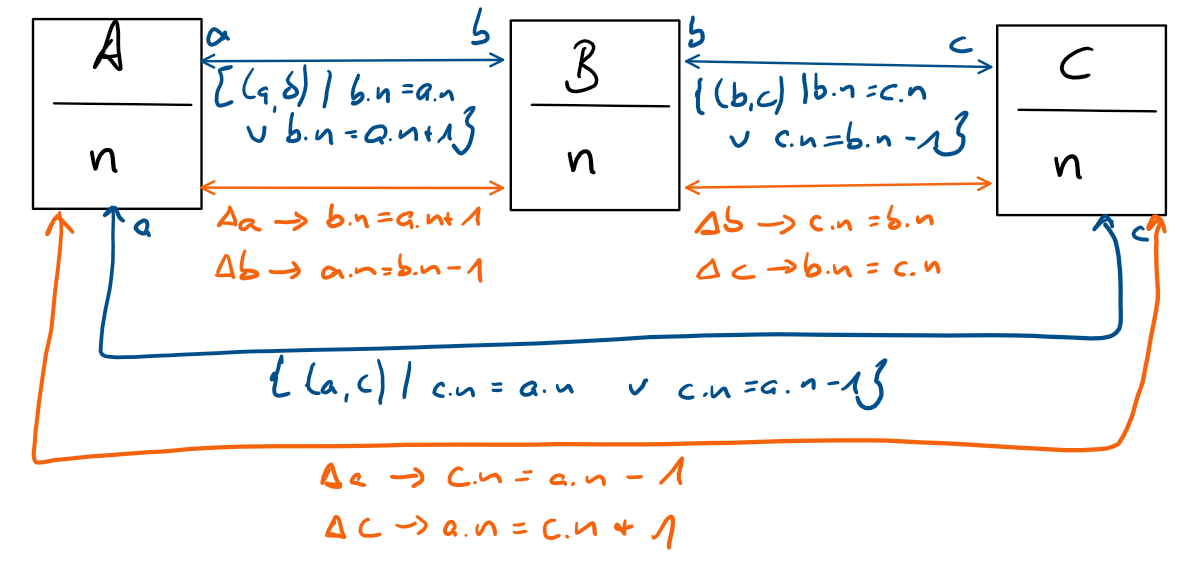
\includegraphics[width=\textwidth]{figures/correctness/formal/divergence_example.png}
    \caption{Example for divergence}
    \label{fig:formal:noexecutionorder}
\end{figure}

\mnote{Restriction to transformations are necessary to decide the orchestration problem}
We will discuss in \autoref{chap:orchestration} in detail whether we can find restrictions for the transformations that ensure that an orchestration that reveals a consistent result always exists.
We will also prove that without further restrictions the decision problem whether an orchestration exists that leads to a consistent result is undecidable.
Due to these degrees of freedom, the definition does not further restrict that an orchestration of transformations has to lead to a consistent result.

\mnote{Application function to make process of applying transformations explicit}
A \gls{orchestration function} does only determine an order of transformations.
Intuitively speaking, consistency for given models and changes to them can be preserved by requesting an orchestration from that function and executing the transformations in the given order.
We make this process explicit by defining an \emph{\gls{application function}} that is able to perform consistency preservation based on given transformations, an orchestration function for them and the actual models and changes.

\mnote{Simplify transformation concatenation by a generalization function}
Before defining that \gls{application function}, we first need to define an auxiliary function to concatenate transformations, more precisely their contained \glspl{consistency preservation rule}.
\Glspl{consistency preservation rule} according to \autoref{def:consistencypreservationrule} are restricted to the two metamodels they are defined for.
Additionally, they require initial models and changes as input, but only return changes.
For these two reasons, the functions describing the preservation rules cannot be easily concatenated.
This, however, is necessary to formally describe their consecutive execution.
We define a \emph{generalization function} for transformations, which generalizes them to arbitrary sets of metamodels and a conforming signature for their input and output, which eases the description of their concatenation.

\begin{definition}[Transformation Generalization Function]
    Let $\transformation{t} = \tupled{\consistencyrelation{CR}, \consistencypreservationrule{\consistencyrelation{CR}{}}}$ be a transformation for metamodels $\metamodel{M}{i}, \metamodel{M}{k}$.
    Let $\metamodeltuple{M} = \tupled{\metamodel{M}{1}, \dots, \metamodel{M}{i}, \dots, \metamodel{M}{k}, \dots, \metamodel{M}{n}}$ be a tuple of metamodels containing $\metamodel{M}{i}$ and $\metamodel{M}{k}$.
    A transformation generalization function $\generalizationfunction{\metamodeltuple{M},\transformation{t}}$ for metamodels $\metamodeltuple{M}$ and transformation $\transformation{t}$ is a function:
    \begin{align*}
        \generalizationfunction{\metamodeltuple{M},\transformation{t}} : (\metamodeltupleinstanceset{M}, \changeuniverse{\metamodeltuple{M}}) \rightarrow (\metamodeltupleinstanceset{M}, \changeuniverse{\metamodeltuple{M}})
    \end{align*}
    It generalizes the \modellevelconsistencypreservationrule $\consistencypreservationrule{\consistencyrelation{CR}{}}$ of transformation $\transformation{t}$ such that it can be applied to changes in $\metamodeltuple{M}$ instead of $\metamodel{M}{i}$ and $\metamodel{M}{k}$, i.e. it applies the changes delivered by $\consistencypreservationrule{\consistencyrelation{CR}{}}$ for the relevant models to the given change tuple.
    Let $\modeltuple{m} \in \metamodeltupleinstanceset{M}$ be a model tuple and $\changetuple{\metamodeltuple{M}} = \tupled{\change{\metamodel{M}{1}}, \dots, \change{\metamodel{M}{i}}, \dots, \change{\metamodel{M}{k}}, \dots, \change{\metamodel{M}{n}}}$ a change tuple.
    We define $\tupled{\change{\metamodel{M}{i}}', \change{\metamodel{M}{k}}'} \equalsperdefinition \consistencypreservationrule{\consistencyrelation{CR}{}}(\model{m}{i}, \model{m}{k}, \change{\metamodel{M}{i}}, \change{\metamodel{M}{k}})$.
    Then the generalization function is defined as:
    \begin{align*}
        \generalizationfunction{\metamodeltuple{M},\transformation{t}}(\modeltuple{m}, \changetuple{\metamodeltuple{M}}) =
        (\modeltuple{m}, \tupled{\change{\metamodel{M}{1}}, \dots, \change{\metamodel{M}{i}}' \concatfunction \change{\metamodel{M}{i}}, \dots, \change{\metamodel{M}{k}}' \concatfunction \change{\metamodel{M}{k}}, \dots, \change{\metamodel{M}{n}}})
    \end{align*}
\end{definition}

% \begin{definition}[\ModelLevelConsistencyPreservationRule Generalization Function]
%     Let $\consistencypreservationrule{\consistencyrelation{CR}{}}$ be a \modellevelconsistencypreservationrule for metamodels $\metamodel{M}{i}, \metamodel{M}{k}$.
%     Let $\metamodeltuple{M} = \tupled{\metamodel{M}{1}, \dots, \metamodel{M}{i}, \dots, \metamodel{M}{k}, \dots, \metamodel{M}{n}}$ be a tuple of metamodels containing $\metamodel{M}{i}$ and $\metamodel{M}{k}$.
%     A \modellevelconsistencypreservationrule generalization function $\cprgeneralizationfunction{\consistencypreservationrule{\consistencyrelation{CR}{}}}$ is a function:
%     \begin{align*}
%         \cprgeneralizationfunction{\consistencypreservationrule{\consistencyrelation{CR}{}}} : (\metamodeltupleinstanceset{M}, \changeuniverse{\metamodeltuple{M}}) \rightarrow (\metamodeltupleinstanceset{M}, \changeuniverse{\metamodeltuple{M}})
%     \end{align*}
%     It generalizes $\consistencypreservationrule{\consistencyrelation{CR}{}}$ such that it can be applied to changes in $\metamodeltuple{M}$ instead of $\metamodel{M}{i}$ and $\metamodel{M}{k}$, i.e. it applies the changes delivered by $\consistencypreservationrule{\consistencyrelation{CR}{}}$ for the relevant models to the given change tuple.
%     Let $\modeltuple{m} \in \metamodeltupleinstanceset{M}$ be a model tuple and $\changetuple{\metamodeltuple{M}} = \tupled{\change{\metamodel{M}{1}}, \dots, \change{\metamodel{M}{i}}, \dots, \change{\metamodel{M}{k}}, \dots, \change{\metamodel{M}{n}}}$ a change tuple.
%     We define $\tupled{\change{m}{i}', \change{m}{k}'} \equalsperdefinition \consistencypreservationrule{\consistencyrelation{CR}{}}(\model{m}{i}, \model{m}{k}, \change{\metamodel{M}{i}}, \change{\metamodel{M}{k}})$.
%     Then the generalization function is defined as:
%     \begin{align*}
%         \cprgeneralizationfunction{\consistencypreservationrule{\consistencyrelation{CR}{}}}(\modeltuple{m}, \changetuple{\metamodeltuple{M}}) =
%         (\modeltuple{m}, \tupled{\change{\metamodel{M}{1}}, \dots, \change{\metamodel{M}{i}}' \concatfunction \change{\metamodel{M}{i}}, \dots, \change{\metamodel{M}{k}}' \concatfunction \change{\metamodel{M}{k}}, \dots, \change{\metamodel{M}{n}}})
%     \end{align*}
% \end{definition}

\mnote{Generalization function is universally defined}
The generalization function is a universally-defined auxiliary function only necessary only necessary to formalize the concepts.
It must neither be defined individually for a specific transformation, nor must it be explicitly specified by a developer of transformations at all.

\mnote{Orchestration or application funciton must deal with unresolvable cases}
Finally, either the orchestration function or an application function must also be able to reflect the cases in which no execution order of transformation can be found that restores consistency.
In accordance to the terminology of \textcite{stevens2020BidirectionalTransformationLargeSoSym}, we call those cases \emph{unresolvable}.
From a theoretical perspective, it does not make a difference whether the orchestration or the application function makes that decision. 
Finally, the orchestration function could also directly be encoded into the application function from a theoretical perspective.
However, from a practical perspective we may want to be able to find an execution order although there is no order that results in a consistent state, to be able to find out why it is not possible to restore consistency, e.g., which transformation induces that problem.

\mnote{An application function is partial and applies transformations}
We define a transformation \gls{application function} that applies transformations to a given set of models and changes according to an order delivered by an \gls{orchestration function}.
This function is partial to allow it to indicate that no result with consistent models could be found.
We indicate those cases with the result $\bot$.

\begin{definition}[Transformation Application Function]
    Let $\transformationset{T}$ be a set of synchronizing transformation for consistency relation $\consistencyrelationset{CR}$ on metamodels $\metamodeltuple{M} = \tupled{\metamodelsequence{M}{n}}$ and $\orcfunction{\transformationset{T}}$ an orchestration function for them.
    A transformation \gls{application function} $\appfunction{\orcfunction{\transformationset{T}}}$ for these rules is a partial function:
    \begin{align*}
        &
        \appfunction{\orcfunction{\transformationset{T}}} : (\metamodeltupleinstanceset{M}, \changeuniverse{\metamodeltuple{M}}) \rightarrow \metamodeltupleinstanceset{M} \cup \setted{\bot}
    \end{align*}
    The function takes a consistent tuple of models and a tuple of changes that was performed on them and returns a changed tuple of models by acquiring changes from the consistency preservation rules in $\consistencypreservationruleset{}$. It is partial, because it is allowed to return $\bot$ especially for inconsistent input models but potentially also in other cases. It has to fulfill the following conditions:
    \begin{align*}
        &
        \forall \modeltuple{m} \in \metamodeltupleinstanceset{M} : \forall \changetuple{\metamodeltuple{M}} = \tupled{\change{\metamodel{M}{1}}, \dots, \change{\metamodel{M}{n}}} \in \changeuniverse{\metamodeltuple{M}} :
        \modeltuple{m} \consistenttomath \consistencyrelationset{CR} \Rightarrow \\
        & \formulaskip
        \big( 
        %\appfunction{\orcfunction{\transformationset{T}}}(\modeltuple{m}, \changetuple{\metamodeltuple{M}}) = \bot \\
        %& \formulaskip 
        %\lor
            \exists \modeltuple{m'} \in \metamodeltupleinstanceset{M} : 
            \appfunction{\orcfunction{\transformationset{T}}}(\modeltuple{m}, \changetuple{\metamodeltuple{M}}) = \modeltuple{m'} \Rightarrow\\
            & \formulaskip \formulaskip
            \exists \transformation{t}_{1}, \dots, \transformation{t}_{m} \in \transformationset{T} :
            \exists \changetuple{\metamodeltuple{M}}' = \tupled{\change{\metamodel{M}{1}}', \dots, \change{\metamodel{M}{n}}'} \in \changeuniverse{\metamodeltuple{M}} :\\
            & \formulaskip \formulaskip \formulaskip
            \orcfunction{\transformationset{T}}(\modeltuple{m}, \changetuple{\metamodeltuple{M}}) = \tupled{\transformation{t}_{1}, \dots, \transformation{t}_{m}} \\
            & \formulaskip \formulaskip \formulaskip
            \land \generalizationfunction{\metamodeltuple{M},\transformation{t}_{1}} \concatfunction \dots \concatfunction \generalizationfunction{\metamodeltuple{M},\transformation{t}_{m}}(\modeltuple{m}, \changetuple{\metamodeltuple{M}}) = (\modeltuple{m}, \changetuple{\metamodeltuple{M}}')\\
            & \formulaskip \formulaskip \formulaskip
            \land \tupled{\change{\metamodel{M}{1}}'(\model{m}{1}), \dots, \change{\metamodel{M}{n}}'(\model{m}{n})} = \modeltuple{m'}
        \big)
    \end{align*}
\end{definition}

\mnote{A weak notion of correctness, because of orchestration undecidability}
While the previous definition does not restrict in which cases $\bot$ and in which an actual tuple of models is returned, we define when we consider an \gls{application function} \emph{correct}.
Correctness can be defined in several ways.
For example, we might say that the function is correct if it always returns a consistent tuple of models when there is an order of transformations that leads to those consistent models.
As we will see later, this is, however, generally impossible, because that decision problem is undecidable.
In consequence, the \gls{orchestration function} and \gls{application function} need to operate conservatively, i.e., return $\bot$ although there might be a sequence of transformations whose application leads to consistent models.
As an alternative, we might require the function to always return consistent models when the \gls{orchestration function} delivers a sequence of transformations whose application leads to a consistent tuple of models.
Since we have to deal with conservativeness anyway, this, however, does not provide any benefits.
In consequence, we define correctness as the property that if a tuple of models is returned, it must be consistent.

\begin{definition}[Transformation Application Function Correctness]
    Let $\appfunction{\orcfunction{\transformationset{T}}}$ be an application function for an orchestration function $\orcfunction{\transformationset{T}}$ for transformations $\transformationset{T}$.
    Let $\consistencyrelationset{CR}$ be the set of \glspl{consistency relation} for which the transformations in $\transformationset{T}$ are defined.
    We say that $\appfunction{\orcfunction{\transformationset{T}}}$ is \emph{correct} if its result is either $\bot$ or consistent to $\consistencyrelationset{CR}{}$:
    \begin{align*}
        &
        \appfunction{\orcfunction{\transformationset{T}}} \mathtext{is correct} \equivalentperdefinition \\
        & \formulaskip
        \forall \modeltuple{m} \in \metamodeltupleinstanceset{M} : \forall \changetuple{\metamodeltuple{M}} = \tupled{\change{\metamodel{M}{1}}, \dots, \change{\metamodel{M}{n}}} \in \changeuniverse{\metamodeltuple{M}} :
        \modeltuple{m} \consistenttomath \consistencyrelationset{CR} \Rightarrow \\
        & \formulaskip
        \appfunction{\orcfunction{\transformationset{T}}}(\modeltuple{m}, \changetuple{\metamodeltuple{M}}) = \bot \lor \appfunction{\orcfunction{\transformationset{T}}}(\modeltuple{m}, \changetuple{\metamodeltuple{M}}) \consistenttomath \consistencyrelationset{CR}
    \end{align*}
\end{definition}
% \begin{definition}[Consistency Preservation Application Function]
%     \todo{Define for transformations instead?}
%     Let $\consistencypreservationruleset{}$ be a set of consistency preservation rules for a set of consistency relations $\consistencyrelationset{CR}$ on metamodels $\metamodeltuple{M} = \tupled{\metamodelsequence{M}{n}}$ and $\consistencyorcfunction{\consistencypreservationruleset{}}$ an orchestration function for the consistency preservation rules.
%     A consistency preservation application function $\consistencyappfunction{\consistencypreservationruleset{}}$ for these rules is a partial function:
%     \begin{align*}
%         &
%         \consistencyappfunction{\consistencyorcfunction{\consistencypreservationruleset{}}} : (\metamodeltupleinstanceset{M}, \changeuniverse{\metamodeltuple{M}}) \rightarrow \metamodeltupleinstanceset{M} \cup \setted{\bot}
%     \end{align*}
%     The function takes a consistent tuple of models and a tuple of changes that was performed on them and returns a changed tuple of models by acquiring changes from the consistency preservation rules in $\consistencypreservationruleset{}$. It is partial, because it is allowed to return $\bot$ especially for inconsistent input models but potentially also in other cases. It has to fulfill the following conditions:
%     \begin{align*}
%         &
%         \forall \modeltuple{m} \in \metamodeltupleinstanceset{M} : \forall \changetuple{\metamodeltuple{M}} = \tupled{\change{\metamodel{M}{1}}, \dots, \change{\metamodel{M}{n}}} \in \changeuniverse{\metamodeltuple{M}} :
%         \modeltuple{m} \consistenttomath \consistencyrelationset{CR} \Rightarrow \\
%         & \formulaskip
%         \big( \consistencyappfunction{\consistencypreservationruleset{}}(\modeltuple{m}, \changetuple{\metamodeltuple{M}}) = \bot \\
%         & \formulaskip 
%         \lor
%             \exists \modeltuple{m'} \in \metamodeltupleinstanceset{M} : 
%             \consistencyappfunction{\consistencypreservationruleset{}}(\modeltuple{m}, \changetuple{\metamodeltuple{M}}) = \modeltuple{m'} \land\\
%             & \formulaskip \formulaskip
%             \exists \consistencypreservationrule{1}, \dots, \consistencypreservationrule{m} \in \consistencypreservationruleset{} : %\\
%             %& \formulaskip \formulaskip
%             \exists \changetuple{\metamodeltuple{M}}' = \tupled{\change{\metamodel{M}{1}}', \dots, \change{\metamodel{M}{n}}'} \in \changeuniverse{\metamodeltuple{M}} :\\
%             & \formulaskip \formulaskip
%             \consistencyorcfunction{\consistencypreservationruleset{}}(\modeltuple{m}, \changetuple{\metamodeltuple{M}}) = \tupled{\consistencypreservationrule{1}, \dots, \consistencypreservationrule{m}} \\
%             & \formulaskip \formulaskip
%             \land \cprgeneralizationfunction{\consistencypreservationrule{1}} \concatfunction \dots \concatfunction \cprgeneralizationfunction{\consistencypreservationrule{m}}(\modeltuple{m}, \changetuple{\metamodeltuple{M}}) = (\modeltuple{m}, \changetuple{\metamodeltuple{M}}')\\
%             & \formulaskip \formulaskip
%             \land \tupled{\change{\metamodel{M}{1}}'(\model{m}{1}), \dots, \change{\metamodel{M}{n}}'(\model{m}{n})} = \modeltuple{m'}
%         \big)
%     \end{align*}
%     We say that $\consistencyappfunction{\consistencyorcfunction{\consistencypreservationruleset{}}}$ is \emph{correct} if its result is either $\bot$ or consistent to $\consistencyrelation{CR}{}$:
%     \begin{align*}
%         &
%         \consistencyappfunction{\consistencypreservationruleset{}} \mathtext{is correct} \equivalentperdefinition \\
%         & \formulaskip
%         \forall \modeltuple{m} \in \metamodeltupleinstanceset{M} : \forall \changetuple{\metamodeltuple{M}} = \tupled{\change{\metamodel{M}{1}}, \dots, \change{\metamodel{M}{n}}} \in \changeuniverse{\metamodeltuple{M}} :
%         \modeltuple{m} \consistenttomath \consistencyrelationset{CR} \Rightarrow \\
%         & \formulaskip
%         \consistencyappfunction{\consistencypreservationruleset{}}(\modeltuple{m}, \changetuple{\metamodeltuple{M}}) = \bot \lor \consistencyappfunction{\consistencypreservationruleset{}}(\modeltuple{m}, \changetuple{\metamodeltuple{M}}) \consistenttomath \consistencyrelationset{CR}
%     \end{align*}
% \end{definition}

% The definition of the application function basically ensures that the function either returns $\bot$ or executes the \modellevelconsistencypreservationrules given by the orchestration function to retrieve a changes tuple of models.
% Actually, we want to have a notion of \emph{correctness}, because the function should not return a tuple of models that is not consistent.

% \begin{definition}[Correct Consistency Preservation Application Function]
%     Let $\consistencypreservationruleset{}$ be a set of consistency preservation rules for a set of consistency relations $\consistencyrelationset{CR}$ on metamodels $\metamodeltuple{M} = \tupled{\metamodelsequence{M}{n}}$ and $\consistencyorcfunction{\consistencypreservationruleset{}}$ an orchestration function for the consistency preservation rules.
%     We say that:
%     \begin{align*}
%         &
%         \consistencyappfunction{\consistencypreservationruleset{}} \mathtext{is correct} \equivalentperdefinition \\
%         & \formulaskip
%         \forall \modeltuple{m} \in \metamodeltupleinstanceset{M} : \forall \changetuple{\metamodeltuple{M}} = \tupled{\change{\metamodel{M}{1}}, \dots, \change{\metamodel{M}{n}}} \in \changeuniverse{\metamodeltuple{M}} :
%         \modeltuple{m} \consistenttomath \consistencyrelationset{CR} \Rightarrow \\
%         & \formulaskip
%         \consistencyappfunction{\consistencypreservationruleset{}}(\modeltuple{m}, \changetuple{\metamodeltuple{M}}) = \bot \lor \consistencyappfunction{\consistencypreservationruleset{}}(\modeltuple{m}, \changetuple{\metamodeltuple{M}}) \consistenttomath \consistencyrelationset{CR}
%     \end{align*}
% \end{definition}

This, in fact, is a rather weak notion of correctness. 
Actually, an \gls{application function} that always return $\bot$ is correct according to that definition.
Due to the fact that the orchestration and application function have to operate conservatively, a binary correctness notion is not that relevant anyway.
Rather the degree of conservativeness and how to improve it is of special interest.
\todo{go on here}


\subsection{Transformation Networks}

\todo{Finally define transformation network as tuple and derive research questions from that}




\mnote{Achieving a correct application function}
The definition of the application function basically ensures that the function either returns $\bot$ or executes the \modellevelconsistencypreservationrules given by the orchestration function to retrieve a changes tuple of models.
It is considered \emph{correct} if it ensures that its result is either $\bot$ or a consistent model tuple by executing the \modellevelconsistencypreservationrules given by the orchestration function.
% A correct application function thus has to ensure that its result is either $\bot$ or a consistent model tuple by executing the \modellevelconsistencypreservationrules given by the orchestration function.
In consequence, the application function can be realized by simply executing the result of the orchestration function and check whether the resulting model tuple is consistent or not and return an appropriate result.
Such a realization is generic and does not depend on the actual consistency preservation rules and orchestration function but represents a generic behavior.
Additionally, this gives an implementation of that function the ability to present a faulty result to the user, which eases finding out why no consistent state was reached.

\mnote{Correctness is not crucial}
Finally, correctness is not crucial, because correctness can easily be achieved by performing any execution of transformations and just ensuring that we terminate at some point in time and then decide whether the resulting models are consistent or not and appropriately deliver the result.

\mnote{How to define an orchestration function that is as optimal as possible?}
The remaining difficulty is how to define an orchestration function that fulfills the definition, i.e., to find a finite sequence of transformations, and also one that improves optimality, as an \emph{optimal} function can never be given.
Although the definition of the orchestration function proposes a closed description of that function, in practice such a function will not have a closed form but will be realized as an algorithm that dynamically decides which transformation to execute next.
Therefore the arising problem is that the length of the sequence to execute is not known a priori. Therefore, we need some abortion criterion. When a consistent result is found, this criterion is easy. But since we do not know whether a sequence exist, we need an abortion criterion that is reasonable and does not cut off the process although a consistent solution could be found, thus reducing optimality.
A simple realization for that algorithm to deliver a finite sequence of transformations would be to define a fixed termination criterion, such as a specific number of transformation executions. However, there is no upper bound for the number of executed transformations necessary to achieve consistency. Still, a fixed number (even 0) could be defined for the number of executed transformations to fulfill the definition. Hence, optimality would be 0 then as a consistent result is never reached. We therefore discuss in the following how to define an appropriate orchestration function and how to optimize it.


\todo{Somewhere here things should be moved to orchestration chapter}

\textbf{Overall Goal:} Find correct orchestration function that improves optimality.

There are two ways to improve optimality of the orchestration function:
\begin{enumerate}
    \item Optimize the orchestration function, i.e., find a good order (probably this is not possible), at least find an order that helps the developer to find problems
    \item Optimize the input, i.e., define requirements to the transformations and their relations representing the input to optimize optimality
\end{enumerate}
\todo{We need an example for that}

Both goes hand in hand, because restrictions to the input can never lead to an orchestration function that always terminates without leading to unsupported relevant cases.

This conform to two approaches:
\begin{enumerate}
    \item Dynamic decision about selected transformation and abortion criteria
    \item Constructive restrictions that ensure that appropriate order is (easily) found
\end{enumerate}

\todo{Application function can be generically defined, orchestration maybe not? We actually want to ensure that both are generic and none of them has to be defined for a specific project.}


\section{Summary}

Central Insights:
\begin{itemize}
    \item In networks, we need compatible consistency relations -> first RQ
    \item In networks, we need synchronizing rather than bidirectional transformations -> second RQ
    \item In networks, we need orchestration functions -> third RQ
    \item Correctness is not the problem, optimality is the problem
    \item We can only check dynamically whether a consistent state was reached due to Halting Problem. We cannot guarantee to always find a consistent state
\end{itemize}





%%% THIS VERSION MAKES ORCHESTRATION ON ITS OWN AND DEFINES THE REQUIREMENTS FOR THAT. IT MAY REQUIRE THE RESULT TO BE CONSISTENT OR NOT
% \begin{definition}[Consistency Preservation Application Function]
%     \todo{Define for transformations instead?}
%     Let $\consistencypreservationruleset{}$ be a set of consistency preservation rules for a set of consistency relations $\consistencyrelationset{CR}$ on metamodels $\metamodeltuple{M} = \tupled{\metamodelsequence{M}{n}}$.
%     A consistency preservation application function $\consistencyappfunction{\consistencypreservationruleset{}}$ for these rules is a partial function:
%     \begin{align*}
%         &
%         \consistencyappfunction{\consistencypreservationruleset{}} : (\metamodeltupleinstanceset{M}, \changeuniverse{\metamodeltuple{M}}) \rightarrow (\metamodeltupleinstanceset{M})
%     \end{align*}
%     The function takes a consistent tuple of models and a tuple of changes that was performed on them and returns a changed tuple of models by acquiring changes from the consistency preservation rules in $\consistencypreservationruleset{}$. It is partial, because it is only defined for consistent input model tuples and may not return a result for all possible changes to any model. It has to fulfill the following conditions:
%     \begin{align*}
%         &
%         \forall \modeltuple{m} \in \metamodeltupleinstanceset{M} : \forall \changetuple{\metamodeltuple{M}} = \tupled{\change{\metamodel{M}{1}}, \dots, \change{\metamodel{M}{n}}} \in \changeuniverse{\metamodeltuple{M}} :
%         \modeltuple{m} \consistenttomath \consistencyrelationset{CR} \Rightarrow \\
%         & \formulaskip
%         \exists \modeltuple{m'} \in \metamodeltupleinstanceset{M} :
%         \modeltuple{m'} = \consistencyappfunction{\consistencypreservationruleset{}}(\modeltuple{m}, \changetuple{\metamodeltuple{M}}) \\
%         %\land \modeltuple{m'} \consistenttomath \consistencyrelationset{CR} \\
%         & \formulaskip
%         \land \exists \consistencypreservationrule{1}, \dots, \consistencypreservationrule{m} \in \consistencypreservationruleset{} : 
%         \exists \changetuple{\metamodeltuple{M}}' = \tupled{\change{\metamodel{M}{1}}', \dots, \change{\metamodel{M}{n}}'} \in \changeuniverse{\metamodeltuple{M}} :\\
%         & \formulaskip \formulaskip 
%         \cprgeneralizationfunction{\consistencypreservationrule{1}} \concatfunction \dots \concatfunction \cprgeneralizationfunction{\consistencypreservationrule{m}}(\modeltuple{m}, \changetuple{\metamodeltuple{M}}) = (\modeltuple{m}, \changetuple{\metamodeltuple{M}}')\\
%         & \formulaskip \formulaskip
%         \land \tupled{\change{\metamodel{M}{1}}'(\model{m}{1}), \dots, \change{\metamodel{M}{n}}'(\model{m}{n})} = \modeltuple{m'}
%     \end{align*}
% \end{definition}


% It is obvious that we can define consistency preservation rules for which no execution order can be specified that returns a consistent tuple of models after certain changes. Consider the example in \autoref{fig:formal:noexecutionorder}. There exists no execution order for any input value that terminates. The transformations will always increase the value, although the defined relations could be fulfilled for the input value, but the transformations never find that solution.

% \begin{figure}
%     \centering
%     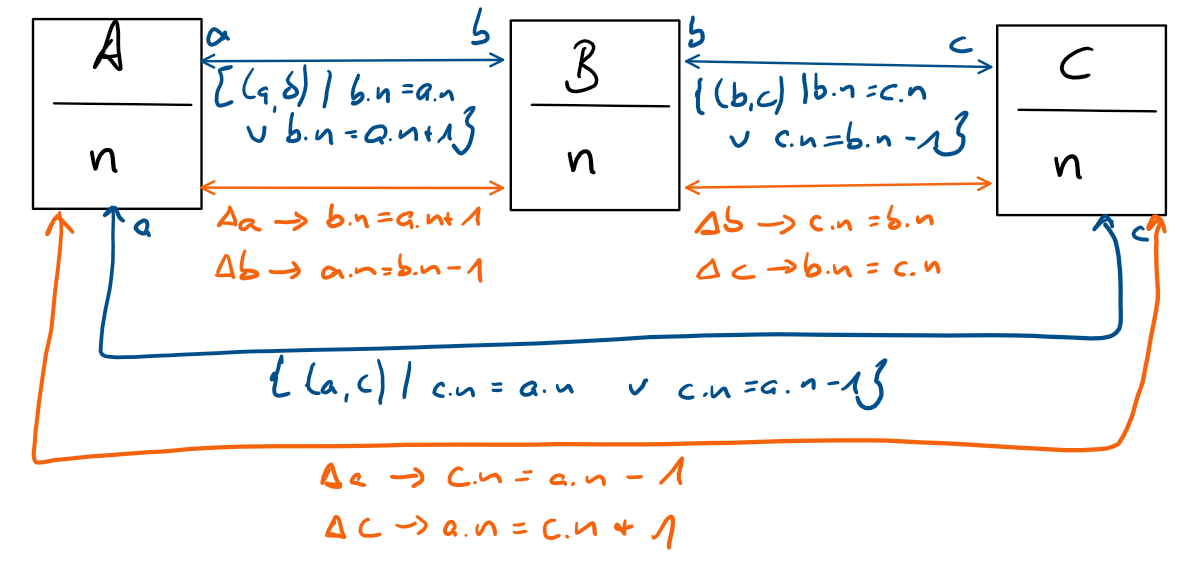
\includegraphics[width=\textwidth]{figures/correctness/formal/divergence_example.png}
%     \caption{Example for divergence}
%     \label{fig:formal:noexecutionorder}
% \end{figure}

% Although we will discuss restrictions to relations and transformations that reduce the chance that no solution can be found, it will not be possible to ensure that such a solution can always be found. This is due to the reason that transformations can perform arbitrary changes given the transformations Turing-completeness, which should not be restricted, because it is unclear which restrictions could be made without forbidding scenarios that should actually we supported. Thus, we assume that transformations are Turing complete.

% Finally, this makes it necessary that a function that applies \modellevelconsistencypreservationrules may not find an execution order that returns a consistent model, thus is should be able to also return $\bot$ as an indicator for that situation.

% We first give a basic definition for such a function without further specifying in which cases the function is expected to return a result other than $\bot$.

% \begin{definition}[Consistency Preservation Application Function]
%     \todo{Define for transformations instead?}
%     Let $\consistencypreservationruleset{}$ be a set of consistency preservation rules for a set of consistency relations $\consistencyrelationset{CR}$ on metamodels $\metamodeltuple{M} = \tupled{\metamodelsequence{M}{n}}$.
%     A consistency preservation application function $\consistencyappfunction{\consistencypreservationruleset{}}$ for these rules is function:
%     \begin{align*}
%         &
%         \consistencyappfunction{\consistencypreservationruleset{}} : (\metamodeltupleinstanceset{M}, \changeuniverse{\metamodeltuple{M}}) \rightarrow (\metamodeltupleinstanceset{M})
%     \end{align*}
%     The function takes a consistent tuple of models and a tuple of changes that was performed on them and returns a changed tuple of models by acquiring changes from the consistency preservation rules in $\consistencypreservationruleset{}$. Thus, it has to fulfill the following conditions:
%     {\setlength{\mathindent}{0em}
%     \begin{align*}
%         &
%         \consistencyappfunction{\consistencypreservationruleset{}}(\modeltuple{m}, \changetuple{\metamodeltuple{M}}) = 
%         \begin{cases}
%             \modeltuple{m'}, & \begin{array}{l@{}}
%                 \exists \changetuple{\metamodeltuple{M}}' = \tupled{\change{\metamodel{M}{1}}', \dots, \change{\metamodel{M}{n}}'} \in \changeuniverse{\metamodeltuple{M}} :\\
%                 \exists \consistencypreservationrule{1}, \dots, \consistencypreservationrule{m} \in \consistencypreservationruleset{} : \\
%                 \cprgeneralizationfunction{\consistencypreservationrule{1}} \concatfunction \dots \concatfunction \cprgeneralizationfunction{\consistencypreservationrule{m}}(\modeltuple{m}, \changetuple{\metamodeltuple{M}}) = (\modeltuple{m}, \changetuple{\metamodeltuple{M}}') \\
%                 \land \tupled{\change{\metamodel{M}{1}}'(\model{m}{1}), \dots, \change{\metamodel{M}{n}}'(\model{m}{n})} = \modeltuple{m'} 
%             \end{array} \\
%             \bot, & otherwise
%         \end{cases}
%     \end{align*}
%     }
% \end{definition}

% \begin{definition}[Consistency Preservation Application Function]
%     \todo{Define for transformations instead?}
%     Let $\consistencypreservationruleset{}$ be a set of consistency preservation rules for a set of consistency relations $\consistencyrelationset{CR}$ on metamodels $\metamodeltuple{M} = \tupled{\metamodelsequence{M}{n}}$.
%     A consistency preservation application function $\consistencyappfunction{\consistencypreservationruleset{}}$ for these rules is function:
%     \begin{align*}
%         &
%         \consistencyappfunction{\consistencypreservationruleset{}} : (\metamodeltupleinstanceset{M}, \changeuniverse{\metamodeltuple{M}}) \rightarrow (\metamodeltupleinstanceset{M})
%     \end{align*}
%     The function takes a consistent tuple of models and a tuple of changes that was performed on them and returns a changed tuple of models by acquiring changes from the consistency preservation rules in $\consistencypreservationruleset{}$. Thus, it has to fulfill the following conditions:
%     {\setlength{\mathindent}{1em}
%     \begin{align*}
%         &
%         \consistencyappfunction{\consistencypreservationruleset{}}(\modeltuple{m}, \changetuple{\metamodeltuple{M}}) = 
%         \begin{cases}
%             \modeltuple{m'}, & \begin{array}{l@{}}
%                 \exists \changetuple{\metamodeltuple{M}}' = \tupled{\change{\metamodel{M}{1}}', \dots, \change{\metamodel{M}{n}}'} \in \changeuniverse{\metamodeltuple{M}} :\\
%                 \exists \consistencypreservationrule{1}, \dots, \consistencypreservationrule{m} \in \consistencypreservationruleset{} : \\
%                 \cprgeneralizationfunction{\consistencypreservationrule{1}} \concatfunction \dots \concatfunction \cprgeneralizationfunction{\consistencypreservationrule{m}}(\modeltuple{m}, \changetuple{\metamodeltuple{M}}) = (\modeltuple{m}, \changetuple{\metamodeltuple{M}}') \\
%                 \land \tupled{\change{\metamodel{M}{1}}'(\model{m}{1}), \dots, \change{\metamodel{M}{n}}'(\model{m}{n})} = \modeltuple{m'} 
%             \end{array} \\
%             \bot, & otherwise
%         \end{cases}
%     \end{align*}
%     }
% \end{definition}



% \begin{definition}[Correct Consistency Preservation Application Function]
%     Let $\consistencyappfunction{\consistencypreservationruleset{}}$ be a consistency preservation application function for a set of \modellevelconsistencypreservationrules $\consistencypreservationruleset{}$ for a set of \modellevelconsistencyrelations $\consistencyrelationset{CR}$.
%     We say that:
%     \begin{align*}
%         &
%         \consistencyappfunction{\consistencypreservationruleset{}} \mathtext{is correct} \equivalentperdefinition \\
%         & \formulaskip
%         \forall \modeltuple{m} \in \metamodeltupleinstanceset{M} : \forall \changetuple{\metamodeltuple{M}} = \tupled{\change{\metamodel{M}{1}}, \dots, \change{\metamodel{M}{n}}} \in \changeuniverse{\metamodeltuple{M}} :
%         \modeltuple{m} \consistenttomath \consistencyrelationset{CR} \Rightarrow \\
%         & \formulaskip
%         \consistencyappfunction{\consistencypreservationruleset{}}(\modeltuple{m}, \changetuple{\metamodeltuple{M}}) \consistenttomath \consistencyrelationset{CR}
%     \end{align*}
% \end{definition}




Now it is obvious that the consistency preservation rules can actually do anything to achieve consistency, including returning always the same set of models that is consistent, although that may not be expected. We will discuss later which reasonable assumptions can be made to the behavior to on the hand not restrict the possibilities of the transformation developer and on the other hand be able to ensure some properties of the transformations and their execution.

\todo{First restriction: Input delta of APP only contains changes to one model -> no synchronisation}
\todo{Second restriction: Input delta is not rejected}
\todo{Third restriction: Generated deltas are monotone}

From a theoretical perspective, it is always possible to a specify consistency relations according to the definition, as it is just a subset of elements.
It is also always possible to define a consistency preservation rule for a consistency relation according to its definition, as can simply return any any element of the relation.
\todo{This is not true: the source model may not be in the relation, then its not possible, at least with the current definition. With a synchronizing transformation, any modification can be made to both models, then its fine.}
The generalization function is generic, so it can always be applied.
Finally, the consistency preservation application function is an artifact that cannot be easily specified according to the definition for a given set of consistency preservation rules.
It is always possible to have a set of consistency preservation rules for which no application function can be defined that returns a consistent result for at least one input model and change tuple, as there is not sequence of consistency preservation rules that achieves that.
\todo{Example!}
Even worse, the problem to define such a function is Turing-complete, which makes it impossible to decide whether such a function exists.
\todo{Show Turing-completeness}
Consequence: From a theoretical perspective, this function is the crucial part!

Essential problem: One transformation may restore consistency between A and B and another between A and C. If then a transformation restores consistency between B and C, the resulting B' and C' may not be consistent A anymore.

Alternative to an app function: Define a \emph{well-definedness} property for a set of transformations, requiring that they can be executed in any order to always terminate consistently. However, this is a very strict requirement, which can usually not be fulfilled, so we do not further investigate that.
\todo{Give simple example why that does not work.}


Best-behaved app function: Whenever there is a sequence of CPRs, the app function finds item. This is still not possible due to Turing-completeness. The function would need to decide whether the network terminates or not.

Only achievable app function is a best-effort (i.e. conservative) function: A function that either returns a consistent set of models or that does return bottom. Not making a statement about how often a correct result is returned in comparison to how often it is possible.

This approach is conservative. The question is then, how high the degree of conservativeness is. In the worst case, a function that always returns bottom would fulfill the definition, but that is not what we want. We want to reduce conservativeness.

Goal: Find a solution in as many cases as possible, abort in the others (conservatively). There are two subgoals to achieve that:
1. Function must be correct, i.e. always terminate (no endless sequence of CPR) and terminate in a consistent state
2. Function must be as less conservative as possible

It is clear that we cannot give a closed function for APP that just by a given change returns a sequence of CPR that results in a consistent state. APP has to be calculated dynamically during execution. Therefore we consider it as an algorithm in the following.


\subsection{Achieving a Correct Application Function}
\todo{These problem cannot occur if a function fulfills the definition, because it always finds a sequence. So the question is how to fulfill the definition.}

It is easy to achieve that the APP function only terminates in a consistent state, because knowing the relations allows to check whether all relations are fulfilled. 
\todo{Need to define that a transformation may not be able to process a specific change? Then there could be inconsistent terminiation because a transformation cannot be executed anymore.}

Problems due to which the function does not terminate: Alternation and Divergence

Alternation: Run through same state twice
Divergence: Always produce new states without reaching a consistent state

Two possibilities to avoid problems:
1. Make assumptions to transformations that avoid them
2. Detect them dynamically and abort


\subsubsection{Avoiding Alternation / Divergence}

Making assumptions that avoid them is rather hard, as we will show in the following.

\paragraph{Idea:} Require monotony to avoid alternation

We would have to relax the definition of transformation to be monotone, because if a transformation is monotone, it may only append information, but this is not always possible, as can be seen in the following example. A monotone transformation must be able to return bottom if it cannot make further changes to restore consistency to the relation.

\begin{definition}[Monotone Transformation]
    Transformation gets models M and deltas D and produces new deltas D'. Taking the union of the original models M and the new models D'(M), then D(M) must be a subset of that, because other elements would have been added and removed afterwards or elements would have been changes once by D and again in a different way by D'.

    Generally, monotony could also mean that only the same complete model state is not passed twice. \todo{Why dont we do that?}
\end{definition}

This would mean that each transformation only appends changes, i.e., if an element was added/removed, the transformation may not do the inverse. The same applies to attribute/reference changes: if an attribute/reference was already changes it may not be changed again.
This way, it is by design impossible to pass through the same state again. Actually, if a monotone transformation returns bottom, the network has to terminate with a failure.
However, this is hard restriction to transformations. It leads to the fact that in some networks that actually have a simple solution no solution is found at all. This can be easily seen at the example in \autoref{fig:formal:monotonycounterexample}. In the example adding "aa" to the left model, any execution order of the transformations leads to the situation that a previous change must be revoked to result in a consistent state. However, it is possible to derive a consistent state for that input change.

\begin{figure}
    \centering
    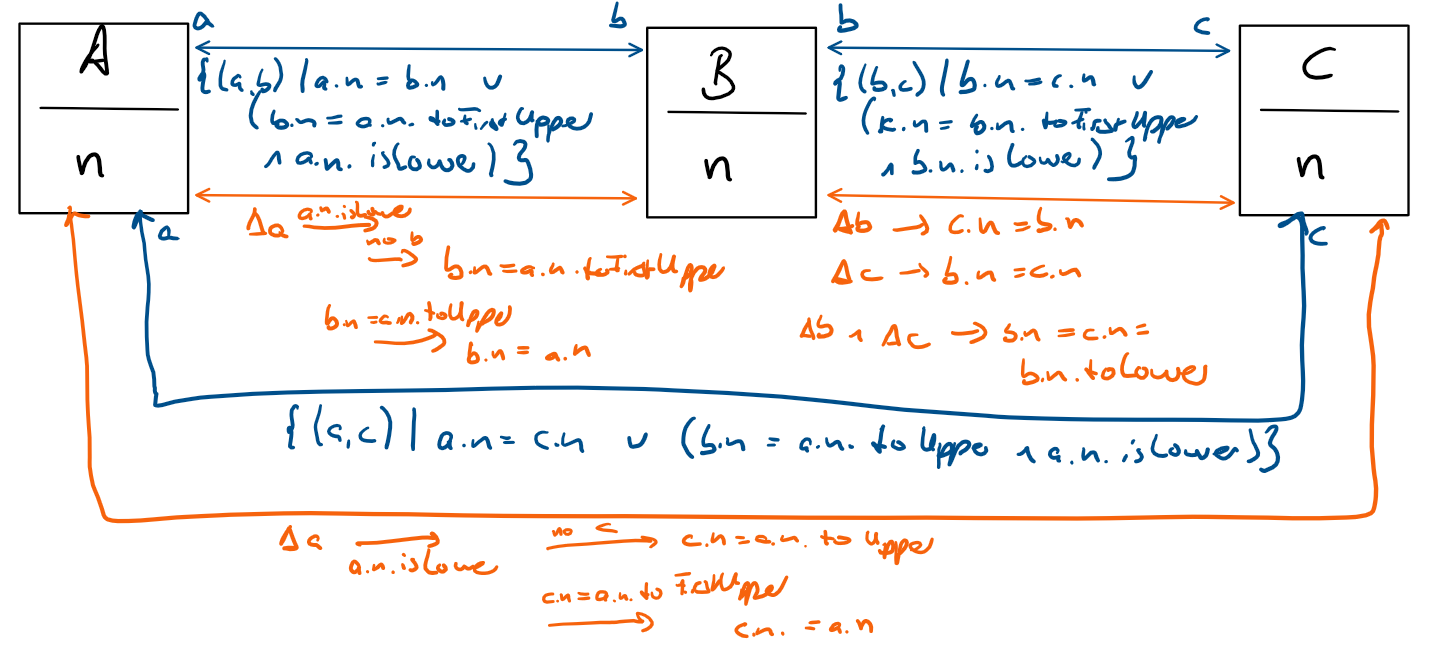
\includegraphics[width=\textwidth]{figures/correctness/formal/monotony_counterexample.png}
    \caption{Counterexample for monotony}
    \label{fig:formal:monotonycounterexample}
\end{figure}

One could now argue that there are binary relations in the example, which may never be fulfilled at all. We will later discuss how far relations that cannot be fulfilled should be restricted. However, in general, this is wanted behavior, because in general it may be necessary that transformations produce intermediate states that are not yet consistent with each other. Otherwise this would means that each transformation is always able to directly deliver a state that is consistent to all other relations, which is especially not possible, because other transformations may add further information to the models. More precisely, a relation may consider <a model consistent to all other models that contain any additional information not affected by the transformation. For example, a UML class model may be considered consistent to all Java models with any implementation of the specified methods, thus to an infinite number of models. Now saying that it should not be allowed that the transformation selects one with an empty implementation because that is not consistent to another relations induced by another transformation, such as the relationship to a component model, does not make any sense. Thus having those relation elements that may be considered locally consistent but will never occur in a globally consistent tuple of models does not make sense.
In the example, we can see that such an inconsistent intermediate state is passed through and afterwards a consistent tuple of models is reached if not requiring monotony.
In consequence, requiring monotony from transformations is a too strict requirement, because it is necessary to run through states that may be changed later on.

\begin{theorem}
    An application function for monotone transformations either returns a consistent model or produce a sequence of CPRs returning delta that return models of always growing size (i.e. it diverges).
\end{theorem}


\paragraph{Divergence cannot be avoided}

There are rather equal network, one that terminates after a long time and one that never terminates. 
Consider the example. The relations are defined in a way such that for any allocation for any of them a consistent tuple of models can be found. However, the transformations are not able to find it because they make "bad" choices from a set of choices that are conflicting. 
This can be seen in the example in \autoref{fig:formal:divergenceexample}.

\begin{figure}
    \centering
    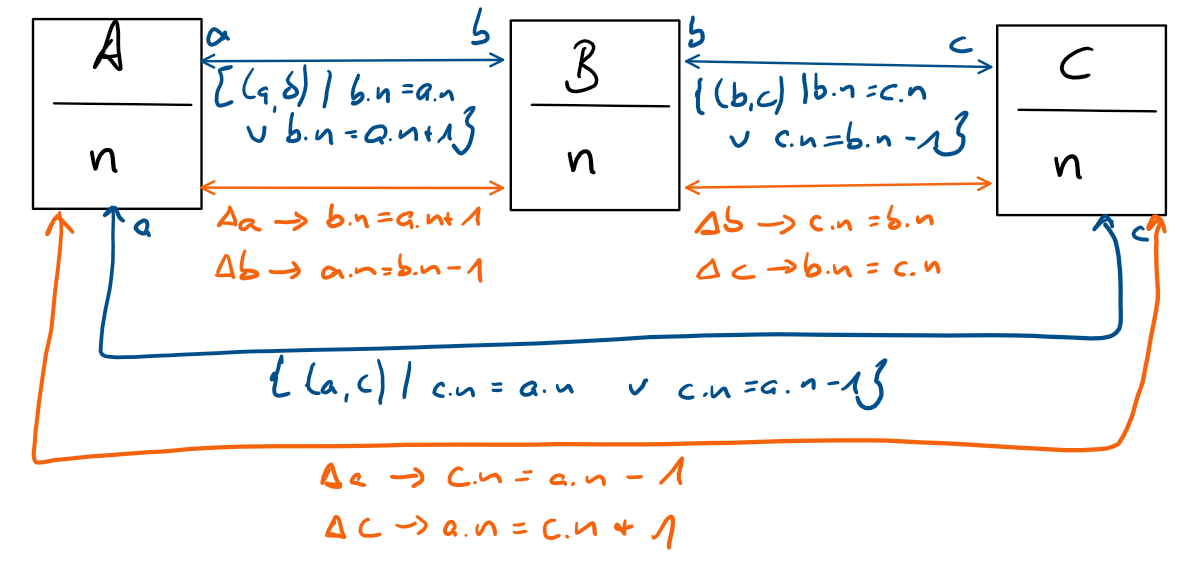
\includegraphics[width=\textwidth]{figures/correctness/formal/divergence_example.png}
    \caption{Example for divergence}
    \label{fig:formal:divergenceexample}
\end{figure}

Thus, systematically avoiding divergence is not possible. 



\paragraph{Detecting Alternation / Divergence}

In consequence, we propose to dynamically deal with alternation / divergence.
To detect alternations, the execution can simply track if a state way already processed. Apart from spatial problems, this does always work.
Finding divergence is not that easy, because it is generally not possible to define an upper bound for the number of executions of a single transformation.
This is due to the reason that, again, this conflicts with the Halting problem.
We can see this at the simple example in \autoref{fig:formal:noupperboundexample}.

\begin{figure}
    \centering
    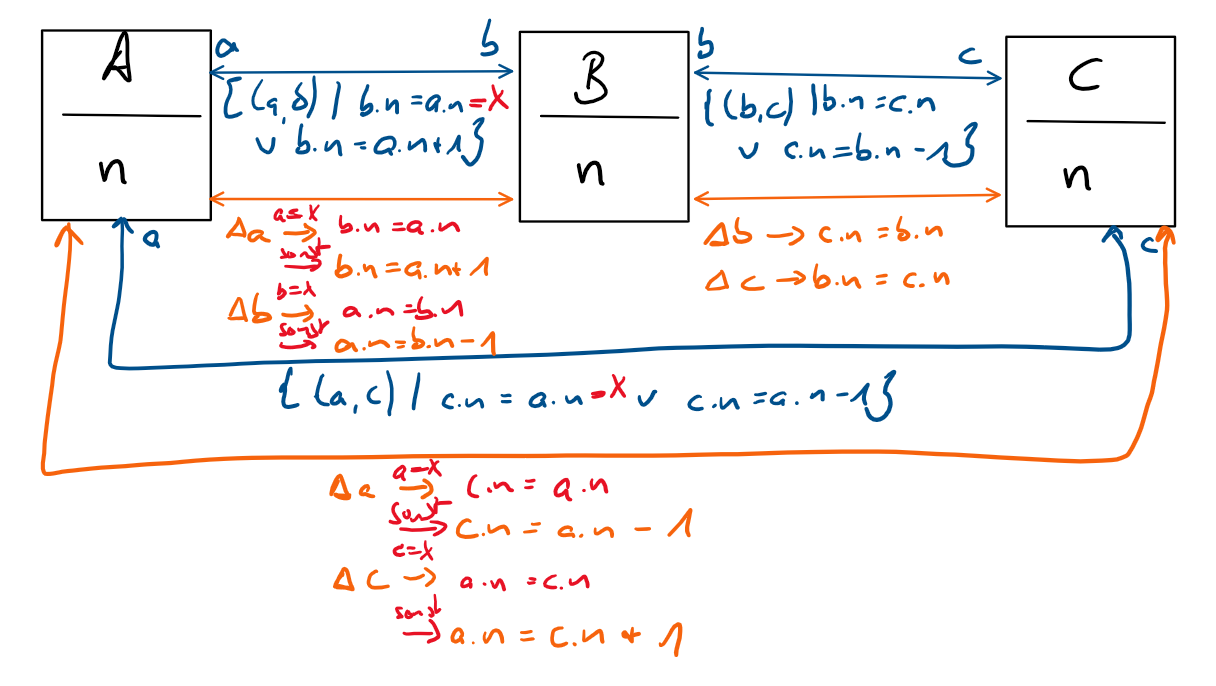
\includegraphics[width=\textwidth]{figures/correctness/formal/no_upper_bound_example.png}
    \caption{Example for no upper bound}
    \label{fig:formal:noupperboundexample}
\end{figure}

Depending on the value X, the transformations have to be executed X times to result in a consistent state. This value can be arbitrarily chosen, thus an arbitrary number of executions may be necessary to terminate in a consistent state.

From an engineering perspective, this is still unwanted behavior. We claim that a transformation network that takes thousands of executions of the same transformation to find a consistent state works not as expected and if running into a failure would expose severe problems to find the reasons for that failures.
Thus, we propose to simply abort the execution after some time to be sure not to run in an endless loop.

Finally, this problem is comparable to ordinary programming, because there the same situations regarding alternation and divergence can occur that result in non-termination of a program.
As we all know, it is impossible to systematically avoid that, but just possible to carefully develop the program and apply best practices to avoid such situations.

In the following, we propose measures to reduce the number of cases in which problematic cases can occur.
In a case study, we will see that using such measures already resolves most of the problems that can occur.
Additionally, we propose an orchestration strategy that improves the possibility to find errors in case something goes wrong.

\textbf{Central insight:} Alternation / Divergence cannot be avoided systematically (like in ordinary programming), if not restricting transformations in a way that may not be reasonable.




\subsection{Reducing Conservativeness of the Application Function}

Goal: Find a solution in as many cases as possible, abort in the others (conservatively). There are two approaches to achieve that: 
1. Reduce the number of cases in which there is no solution by adding assumptions to the relations and transformations (restrict input of app function)
2. Improve the ability to find a solution if it exists (improve capabilities of app function)
Secondary goal: In cases, in which no solution is found, support the user in understanding why no solution was found.


Regarding 1: Reduce problematic cases


1. reduce cases in which there is no such solution
1.1. On relation level: Only sets, so analysis possible.
Ensure that relations are defined in a way such that they do not allow a locally correct set of CPRs that has no APP solution. If there is a pair of models (or elements of a fine-grained relation) in a relation, a CPR may return it. But if there is no consistent tuple of models containing these two, it does not make any sense to consider these elements (even worse, if we have monotony, adding these elements makes the network unsolvable). For that reason, we need compatibility. Avoids both alternation and divergence
1.2. On transformation level: Hard to perform analyses
Require monotony to avoid alternation
Give some example why divergence cannot easily be avoided, thus terminate at some point
2. find the solution in as many cases as possible -> reasonable orchestration strategy
Focus on engineering solution 


Thus, there arise two questions:
- Although theoretically easy, how to practically define a CPR that is synchronizing?
- How to define an APP function and which requirements does that impose?












Two levels of correctness:
\begin{enumerate}
    \item Local correctness: a consistency relation is correct to the global relation and the CPR is to the relation, i.e. given two models and changes in them, the transformation can produce a change that restores consistency regarding the global consistency relation of these two models (i.e. there are some other models with which these two models would be consistent regarding the global specification) --> a network is locally correct, if this property is fulfilled
    \item Global correctness: the binary relations together are equal to the global one and the execution function is able to find consistency models after a change to initially consistent models --> network is globally correct, if this property is fulfilled
\end{enumerate}
Potentiell ist lokale Korrektheit (zumindest einer CPR zu ihrer CR per Konstruktion) herstellbar -- das war auch das Ergebnis bisheriger Studien --, eventuell auch von einer CR zu einer globalen CR, obwohl die ja eigentlich meist nicht existiert, daher nehmen wir das als gegeben an.
Dann zeigen, dass die globale Beziehung der Relationen nicht äquivalent ist zu den einzelnen lokalen, daher kommt hier zusätzliche Komplexität rein (Kompatibilitätsbegriff).
Final muss noch die Ausführungsfunktion korrekt sein, hier aber Problem der Turing-Vollständigkeit. 
Daher Einschränkungen an Transformationen finden bzw. ingenieurmäßige Ausführungsreihenfolge festlegen, die möglichst oft richtige Lösungen findet und sonst konservativ mit einem Fehler terminiert.


\textbf{On top of ordinary bx correctness:}
\begin{itemize}
    \item Transformations need to be synchronizing
    \item Consistency relations need to fulfill a notion of correctness
    \item Exkurs:
    \begin{itemize}
    \item Is compatibility a subclass of correctness? Is every correct set of relations compatible as well?
    \item Problematisch: unser Konsistenzbegriff für Relationen (feingranulare Relationen) schließt keine Modelle aus, der Konsistenzbegriff hier aber schon. Wie realisiere ich die feingranularen Relationen, die dafür sorgen, dass nur genau ein Tupel von Modellen konsistent ist?
    \item Wir müssen bei der Ableitung unseres Kompatibilitätsbegriffes erklären, dass bei uns der vollständige Ausschluss bestimmter Modelle nicht Teil einer feingranularen Konsistenzrelation sein darf, sondern Teil einer weiteren Spezifikation, die angibt, welche Modelle überhaupt valide sind. Denn so ist es in Transformationssprachen tatsächlich auch.
    \end{itemize}
    \item Execution function needs to be defined, which potentially induces requirements to the transformations.
\end{itemize}


Annahmen:
\begin{itemize}
    \item Nutzeränderungen dürfen nicht rückgängig gemacht werden.
    \item Nutzeränderungen lassen sich so feingranular zerlegen, dass, falls durch die Erzeugung/Änderung eine Konsistenzrelation verletzt wird, es in jeder unabhängigen Teilmenge von Konsistenzrelationen eine verletzte Konsistenzrelation gibt, für die die geänderten Elemente einem Condition Elemente entsprechen, es also insbesondere keine Teilmenge der geänderten Element gibt, die bereits dieses Condition Element sind. Ansonsten ist durch unsere Kompatibilitäts-Definition nicht sichergestellt, dass eine konsistente Modellmenge gefunden werden kann.
\end{itemize}

Voraussetzungen:
\begin{itemize}
    \item Relationen müssen korrekt sein, d.h. sie müssen bzgl. einer globalen (meist eher implizit bekannten) n-ären Relation zwischen allen Modellen identisch sein. Eine n-äre Relation lässt sich nicht immer zerlegen (siehe Stevens), aber wir nehmen das an.
    \item Die einzelne Transformation muss bzgl. ihrer Relation korrekt sein, d.h. sie muss bei Änderungen in beiden Modellen ein zur Relation konsistentes Modell liefern.
\end{itemize}

Ebenen der Korrektheit:
\begin{itemize}
    \item Relationen müssen korrekt sein, d.h. gegeben eine Nutzeränderung muss es überhaupt möglich sein eine konsistente Menge an Modellen zu finden. Wenn Transformationen etwas beliebigen tun dürfen geht das immer. Wir nehmen an, dass eine Nutzeränderung nicht rückgängig gemacht werden soll (bzw. wenn sie rückgängig gemacht werden würde eigentlich die Änderung invalide war, d.h. keine Konsistenz im Netzwerk hergestellt werden kann). Daher sind Relationen nur korrekt, wenn für fixierte Elemente, die durch eine Nutzeränderung entstehen können, eine Modellmenge abgeleitet werden kann, die bzgl. der Relationen konsistent ist. D.h. gegeben einige Elemente muss es eine Modellmenge geben, die in allen Relationen liegt und die diese Elemente enthält (-> Kompatibilitätsbegriff). Wir betrachten in Kapitel ?, wie man Kompatibilität präzise definieren und feststellen/garantieren kann.\\
    Resultat: Gegeben eine Änderung ist es möglich eine Transformation anzugeben, die aus der Änderung ein konsistentes Modell produziert.
    \item Einzelne Transformationen müssen korrekt sein: Wir fordern Korrektheit der Transformation sowieso. Allerdings machen in einem Netzwerk verschiedene Transformationen Änderungen an allen Modellen, d.h. wir müssen nicht den "normalen" Transformationsfall unterstützen, dass Deltas in einem Modell ins andere übertragen werden, um Konsistenz herzustellen, sondern die Transformationen müssen \emph{synchronisierend} sein, also Deltas in beiden Modelle annehmen und dann Konsistenz herstellen. Wir definieren diese Synchronisationseigenschaft und betrachten in Kapitel ?, welcher zusätzlichen Anforderungen sich dadurch bzgl. EMOF-Modellen ergeben. Der Input sind Deltas in zwei Modellen, und einzelne Deltas sind potentiell als "authoritative" definiert, was bedeutet, dass die erzeugten/geänderten Elemente nicht noch einmal geändert/gelöscht werden dürfen. Das realisiert die Anforderung, dass Nutzeränderungen nicht rückgängig gemacht werden dürfen. \\
    Resultat: Gegeben Änderungen in zwei Modellen (mit potentiell authoritativen Änderungen) gibt die Transformation ein konsistentes (bzgl. der Konsistenzrelation) Modellpaar zurück. 
    \item Korrektheit der Anwendungsfunktion: Die Anwendungsfunktion muss die Transformationen in einer 
\end{itemize}

Annahme an Transformationen:
\begin{itemize}
    \item Muss eine Transformation mit jedem beliebigen Delta umgehen können müssen? Eine Einschränkung auf Monotonie würde dies verhindern. Bzw. wir müssten zeigen, dass es Konsistenzrelationen gibt, die unter der Anforderung an Monotonie nicht wiederhergestellt werden können. Bspw. fügt eine andere Transformation 3 Elemente hinzu, wo zwei mit dem anderen entsprechend der Konsistenzrelationen korrelieren und somit keine Witness-Struktur aufgebaut werden kann, die Konsistenz beweist. Das lässt sich durch Hinzufügen weiterer Elemente potentiell nicht auflösen (siehe Beispiele im SoSym-Paper).
\end{itemize}

\todo{Überlegen, wo hier die Definition von (undirektionalen Relationen) rein muss.}
Präzisere Eigenschaften:
\begin{itemize} 
    \item Synchronisationseigenschaft: Eine Transformation kann mit Änderungen an mehreren Modellen umgehen, d.h. gegeben zwei konsistente Modelle + Änderungen an beiden resultiert in zwei Modellen, die konsistent bzgl. der Relation(en) zwischen den Metamodellen sind
    \item 
\end{itemize}  

\begin{itemize}
    \item Kompatibilität entsprechend Modularisierungsebene
    \item Synchronisation auf Operationalisierungsebene: Abwägen, dass eine Transformation verschiedene Zustände sehen könnte, auf denen sie ausgeführt wird. Aber letztendlich muss sie damit klarkommen, dass zwei Modelle geändert wurden. 
\end{itemize}

TODO:
\begin{itemize}
    \item Authoritative Modelle (bzw. eher authoritative Regionen) diskutieren (Verweis Stevens)
\end{itemize}



\section{Local Correctness}

Simple solution: we define a transformation which normatively implies a relation, thus it is correct by construction. From a theoretical perspective this is easy to reach, from a practical it is not.
However, in contrast to our definition of synchronizing transformations, ordinary transformations are only able to process changes in one model and update the other accordingly. Together with the assumption that both models were consistent before does not fit with our scenario, because if one model is modified, the other may be modified as well by another transformation across another path, before a transformation is executed. Thus, both models may have been modified.
We consider the following situation: Models A and B were consistent. Model A was changed an we have the changes at hand. Additionally, B was modified because there were other changes propagated through the network. 
We distinguish all cases of modifications to B that may have violated a consistency relation between A and B (according to our fine-grained consistency notion) and consider what we have to do there (e.g. find-or-create-pattern).
Put empirical analysis here.


\section{Correct APP function}

We make the following approach: Always assume there is a solution and start executing the transformation (for now in any order). Finally, the network has to terminate at a fixed point. We investigate, what the reasons may be that it does not try to avoid them.

These reasons can lie in the relations:
- relations cannot be completely unfulfillable, as the empty models are always consistent, thus there can always be CPRs that result in a consistent set of models
- however, if relations contain pairs that can never be in any consistent model tuple they improve proneness to errors, because a CPR may return that pair, which will never fit to any result of any other transformation. Thus, this should not be allowed -> compatibility

These reasons can also lie in the transformations:
- Transformations can make choices and they make choices that are always incompatible to other (refer to example)

Essentially there are two problems: alternation and divergence



\subsection{Other thought}
If each element occurs in each relation only once (so always 1:1 mappings) and if we have compatibility, then any transformation order would return exactly the one model tuple that fits.
However: In that case we would have confluence, every information must directly be available in B from A without a transitive propagation over C. This is not what we want. So there must in general be more than one option a transformation is fine with that to reflect the information that another transformation may add or change.


\todo{Hippocraticness is not necessary but needs to be discussed}

Goal:
- Find a solution in as much cases as possible, abort in the others (conservatively)
- To do so: reduce cases in which there is no such function
- To do so: ensure that relations are defined in a way such that they do not allow a locally correct set of CPRs that has no APP solution. If there is a pair of models (or elements of a fine-grained relation) in a relation, a CPR may return it. But if there is no consistent tuple of models containing these two, it does not make any sense to consider these elements (even worse, if we have monotony, adding these elements makes the network unsolvable). For that reason, we need compatibility.
- 
